\documentclass[11pt]{article}

% --- Core packages & order ---
% math text & symbols
\usepackage{amsmath,amssymb}
% define \texorpdfstring (load late is safest)
\usepackage[hidelinks]{hyperref}
\usepackage[T1]{fontenc}
\usepackage{lmodern}
\usepackage[margin=1in]{geometry}
\usepackage{microtype}
\usepackage{xcolor}
\usepackage{graphicx}          % for \resizebox
\graphicspath{{figures/}}
\usepackage{booktabs}
\usepackage{tabularx,makecell,array}
\usepackage{multicol}
\usepackage{enumitem}
\usepackage{parskip}
\usepackage{ellipsis} % improves spacing around \dots/\ldots automatically
\usepackage{tabularx}
\usepackage{tikz}              % load TikZ first...
\usetikzlibrary{arrows.meta,calc,positioning}  % ...then libraries

\usepackage{subcaption}
\usepackage{needspace}
\usepackage{float}
\usepackage{placeins}

% --- Color palette ---
\definecolor{royal}{RGB}{12,64,145}
\definecolor{sanctum}{RGB}{0,120,80}
\definecolor{ink}{RGB}{30,30,30}
\definecolor{ccol}{RGB}{55,110,180}
\definecolor{scol}{RGB}{120,60,160}
\definecolor{rocol}{RGB}{220,130,40}
\definecolor{rccol}{RGB}{190,40,50}
\definecolor{capcol}{RGB}{60,140,80}

% --- tcolorbox (load once, after colors) ---
\usepackage[most]{tcolorbox}

% --- Small UI helpers (now safe because TikZ is loaded) ---
\newcommand{\CrownIcon}{%
  \tikz[baseline=-0.5ex,scale=0.14]{
    \fill[orange!70!yellow] (0,0) -- (0.65,0.9) -- (1.3,0) -- (1.95,0.9) -- (2.6,0) -- cycle;
    \fill[orange!80!brown]  (0,-0.36) rectangle (2.6,0);
  }%
}

% --- Optional badge & variant box (uses tcolorbox) ---
% Pill that pops on a dark title bar
\newtcbox{\optbadgeOnDark}{on line, arc=4pt, boxrule=0pt,
  colback=orange!70!yellow, colframe=white,
  left=4pt, right=4pt, top=1pt, bottom=1pt, boxsep=1.5pt,
  tcbox raise base, fontupper=\scriptsize\bfseries\color{black}}
  

\newtcolorbox{rulevariant}[1][]{%
  enhanced, breakable,
  colback=royal!3, colframe=royal!70!black, boxrule=0.8pt,
  rounded corners, left=7pt, right=7pt, top=7pt, bottom=7pt,
  coltitle=white,
  attach boxed title to top left={yshift=-2mm, xshift=3mm},
  boxed title style={colback=royal!85!black, colframe=royal!85!black},
  fonttitle=\bfseries,
  title={\CrownIcon\;Crown Buyback\;\optbadgeOnDark{OPTIONAL}},
  #1}

% --- Table/layout tweaks ---
\setlength{\columnsep}{0.75em}
\setcounter{tocdepth}{2}
\setcounter{secnumdepth}{2}
\newcolumntype{Y}{>{\raggedright\arraybackslash}X}
\setlength{\tabcolsep}{6pt}
\renewcommand{\arraystretch}{1.15}
\setlength{\parindent}{0pt}

% --- Status badges (TEXT mode; do not put them in \( ... \)) ---
\newcommand{\CC}[1]{\textcolor{blue!60!black}{\scriptsize\ttfamily[CF:#1]}}
\newcommand{\SC}[1]{\textcolor{red!60!black}{\scriptsize\ttfamily[S:#1]}}
\newcommand{\RoC}{\textcolor{teal!60!black}{\scriptsize\ttfamily[Rooted]}}
\newcommand{\RC}{\textcolor{purple!70!black}{\scriptsize\ttfamily[RC]}}
\newcommand{\CapC}[1]{\textcolor{green!40!black}{\scriptsize\ttfamily[G:#1]}}

% --- Thought helper ---
\newcommand{\think}[1]{\emph{\footnotesize #1}}

% =========================
% Board config + TikZ styles
% =========================
\newcommand{\BoardN}{8}               % board size (NxN)
\newcommand{\SanctumA}{1/4}           % left side-apex Sanctum
\newcommand{\SanctumB}{8/5}           % right side-apex Sanctum

\tikzset{
  sq/.style={draw, line width=0.3pt},
  cross/.style={fill=blue!22},      % center Cross (2x2)
  apexA/.style={fill=green!18},     % top apex square
  apexB/.style={fill=green!26},     % bottom apex square
  sanctumA/.style={fill=red!28},    % left Sanctum
  sanctumB/.style={fill=red!34},    % right Sanctum
  zoc/.style={fill=black!18},
  moveArrow/.style={-Latex, line width=0.8pt},
  piece/.style={circle, draw, fill=white, line width=0.8pt, minimum size=7.5pt, inner sep=0pt}
}

% Grid + shading (top-left origin: physical y = BoardN - y)
\newcommand{\DrawGrid}{%
  \foreach \x in {1,...,\BoardN}{%
    \foreach \y in {1,...,\BoardN}{%
      \pgfmathtruncatemacro{\yphys}{\BoardN-\y}%
      \pgfmathtruncatemacro{\shade}{mod(\x+\y,2)==0 ? 3 : 0}%
      \fill[black!\shade] ({\x-1},{\yphys}) rectangle ++(1,1);
      \draw[sq] ({\x-1},{\yphys}) rectangle ++(1,1);
    }%
  }%
}
\newcommand{\ShadeSquares}[2]{% #1=style, #2="x/y,x/y,..."
  \foreach \x/\y in {#2}{%
    \pgfmathtruncatemacro{\yphys}{\BoardN-\y}%
    \path[#1] ({\x-1},{\yphys}) rectangle ++(1,1);
  }%
}
\newcommand{\ShadeCross}[1]{%
  \pgfmathtruncatemacro{\L}{\BoardN/2}%
  \pgfmathtruncatemacro{\H}{\L+1}%
  \foreach \x/\y in {\L/\L,\L/\H,\H/\L,\H/\H}{%
    \pgfmathtruncatemacro{\yphys}{\BoardN-\y}%
    \path[#1] ({\x-1},{\yphys}) rectangle ++(1,1);
  }%
}
\newcommand{\RedrawGridLines}{%
  \foreach \x in {1,...,\BoardN}{%
    \foreach \y in {1,...,\BoardN}{%
      \pgfmathtruncatemacro{\yy}{\BoardN-\y}%
      \draw[sq] ({\x-1},{\yy}) rectangle ++(1,1);
    }%
  }%
}

% Cardinal labels used in your minis (adjust as you prefer)
\newcommand{\LabelN}{OR}
\newcommand{\LabelE}{OL}
\newcommand{\LabelS}{HR}
\newcommand{\LabelW}{HL}

% Piece placers (safe now that TikZ is loaded)
\newcommand{\PlaceA}[3]{\pgfmathtruncatemacro{\yphys}{\BoardN-#3}\node[piece,fill=white,text=black] at ({#2-0.5},{\yphys+0.5}) {\scriptsize\bfseries #1};}
\newcommand{\PlaceB}[3]{\pgfmathtruncatemacro{\yphys}{\BoardN-#3}\node[piece,fill=black,text=white] at ({#2-0.5},{\yphys+0.5}) {\scriptsize\bfseries #1};}

% ==== Directional move notation (robust) ====
% Usage: \On[OL]{2}, \On[OR]{3}, \Hm[HL]{1}, \Hm[HR]{2}
\makeatletter
\newcommand{\KR@OnPretty}[1]{%
  \def\tmp{#1}\def\OL{OL}\def\OR{OR}%
  \if\relax\detokenize{#1}\relax\else
    \ifx\tmp\OL L\else\ifx\tmp\OR R\else #1\fi\fi
  \fi
}
\newcommand{\KR@HmPretty}[1]{%
  \def\tmp{#1}\def\HL{HL}\def\HR{HR}%
  \if\relax\detokenize{#1}\relax\else
    \ifx\tmp\HL L\else\ifx\tmp\HR R\else #1\fi\fi
  \fi
}
\newcommand{\KR@MoveCore}[3]{%
  \mbox{\textsc{#1}\if\relax\detokenize{#2}\relax\else$_{\mathrm{#2}}$\fi\,\textbf{#3}}%
}
% Force (re)define even if a 1-arg legacy \On/\Hm exists
\DeclareRobustCommand{\On}[2][]{\KR@MoveCore{on}{\KR@OnPretty{#1}}{#2}}
\DeclareRobustCommand{\Hm}[2][]{\KR@MoveCore{hm}{\KR@HmPretty{#1}}{#2}}
\makeatother

% === Faction blurb block (name + one-line desc + optional tagline) ===
% Usage:
%   \factionblurb{Ykrul (Kon'reh)}{Control-first pragmatists...}{“Count exits, not victims.” — Kargath}
%   \factionblurb{Ecktorian}{Engineers of symmetry...}{}   % <- no tagline line
\newcommand{\factionblurb}[3]{%
  \par\medskip
  \Needspace{3\baselineskip}% keep label+desc+tagline together when possible
  \noindent\textbf{#1. }#2\par
  \smallskip
  \if\relax\detokenize{#3}\relax\else\emph{#3}\par\fi
}

% ==== Simple Coach's Notes (no tables) ====
\newtcolorbox{coachbox}[1]{%
  enhanced, breakable,
  colback=royal!3, colframe=royal!70!black, boxrule=0.8pt,
  rounded corners, left=7pt, right=7pt, top=7pt, bottom=7pt,
  coltitle=white,
  attach boxed title to top left={yshift=-2mm, xshift=3mm},
  boxed title style={colback=royal!85!black, colframe=royal!85!black},
  fonttitle=\bfseries,
  title={#1}, before skip=6pt, after skip=6pt, width=\linewidth,
}

% Coach’s Notes environment: uses description list for Cue → Note
\newenvironment{coachnotes}[1]{%
  \begin{coachbox}{#1}%
    \footnotesize
    \begin{description}[leftmargin=2.8cm,labelsep=0.6em,font=\scshape,
                        itemsep=0.25em,parsep=0pt,topsep=0.2em]
}{%
    \end{description}%
  \end{coachbox}%
}

% Convenience macro for rows
\newcommand{\CNRow}[2]{\item[#1] #2}

% --- helpers (safe: only define if missing) ---
\providecommand{\playdesc}[1]{\par\smallskip\noindent\small\textbf{Play.} #1\par}
\newcommand{\flavline}[2]{\noindent\textbf{#1.} \textit{#2}\par}

% --- Engine-log friendly wrappers (reuse \On and \Hm) ---
% LANE: pass L or R (OL/OR/HL/HR still OK via your pretty-mapper)
\makeatletter

% convenience tags
\newcommand{\CFIn}[1]{\CC{in #1/3}}
\newcommand{\CFOut}{\CC{out}}

% allow \RC both bare and with a count: \RC  or  \RC[3/5]
\renewcommand{\RC}[1][]{%
  \textcolor{purple!70!black}{\scriptsize\ttfamily[RC%
  \if\relax\detokenize{#1}\relax\else~#1\fi]}}

% verb dispatchers -> your existing \On / \Hm
\expandafter\def\csname mvverb@on\endcsname#1#2{\On[#1]{#2}}
\expandafter\def\csname mvverb@hm\endcsname#1#2{\Hm[#1]{#2}}

% specials (no lane/step)
\expandafter\def\csname mvverb@H\endcsname#1#2{{\SC{H}}}      % Hop-capture tag
\expandafter\def\csname mvverb@D\endcsname#1#2{{\SC{D}}}      % Displacement tag
\expandafter\def\csname mvverb@seed\endcsname#1#2{{\textsc{seed}}}

% directional move: \mv[Side]{Piece}{verb}{Lane}{Steps}{tail}
\DeclareRobustCommand{\mv}[6][]{%
  \if\relax\detokenize{#1}\relax\else\textbf{#1:}\ \fi
  \textbf{#2}\ %
  \csname mvverb@#3\endcsname{#4}{#5}%
  \if\relax\detokenize{#6}\relax\else\ #6\fi
}

% special-only (no lane/steps): \mvs[Side]{Piece}{Special}{tail}
\DeclareRobustCommand{\mvs}[4][]{%
  \if\relax\detokenize{#1}\relax\else\textbf{#1:}\ \fi
  \textbf{#2}\ %
  \csname mvverb@#3\endcsname{}{ }%
  \if\relax\detokenize{#4}\relax\else\ #4\fi
}
\makeatother

\begin{document}\color{ink}

%==============================
% Title Page
%==============================
\begin{titlepage}
  \thispagestyle{empty}
  \begin{center}
    \vspace*{1.5cm}

    {\Huge \bfseries KON'REH}\\[8pt]
    {\Large Core Rules}\\[2pt]
    {\large and Lore Compendium}\\[20pt]

    \rule{0.6\linewidth}{0.6pt}\\[10pt]
    {\large A Game of Apex, Sanctum, and Reforge}\\
    \rule{0.6\linewidth}{0.6pt}\\[22pt]

    {\Large \textit{by} Nicholas A. Gasper}\\[4pt]
    {\normalsize Setting \& Lore by Nicholas A. Gasper}\\[16pt]

    % Optional crest or emblem
    %\vspace{6mm}
\IfFileExists{fig/konreh-crest.png}{%
  \includegraphics[
    width=0.28\linewidth,
    keepaspectratio,
    trim=8 8 8 8,clip
  ]{fig/konreh-crest.png}\par\vspace{8pt}%
}

\end{center}
\end{titlepage}

\pagenumbering{roman}
\tableofcontents
\clearpage

%==============================
% Copyright / Legal Page
%==============================
\clearpage
\thispagestyle{empty}
\vspace*{2cm}

{\small
\noindent \textbf{KON'REH} and associated setting terms including but not limited to:
\textit{Canray}, \textit{K’thra}, \textit{Kanry}, \textit{Twin Apex Seed}, \textit{Reforge},
the names of cultures (e.g., Ykrul, Ecktorian, Vhasian, Viterran, Aeler, Vilikari, Thepyrgosi (Thepyric), Ubral, Silkstrand),
proper nouns, places, characters, flavor quotes, worldbuilding lore, diagrams, iconography,
and the specific textual expression of rules, examples, and notation in this book are
© \the\year\ \textit{Nicholas A. Gasper}. All rights reserved.\\[8pt]

\noindent \textbf{Mechanics Disclaimer.}
The underlying game mechanics, procedures of play, and functional systems described herein are
not claimed as proprietary subject matter. No copyright is asserted in the \emph{ideas} of movement rates,
zones of control, countdowns, or other rules mechanics \emph{as mechanics}; copyright subsists in the
\emph{expression} of those ideas in this book (text, arrangement, examples, graphics, naming, and lore).\\[8pt]

\noindent \textbf{Trademarks.}
KON'REH and other marks herein may be trademarks or registered trademarks of their respective owners.
Use of the marks does not imply endorsement.\\[8pt]

\noindent \textbf{Fan Content Policy (Non-Commercial).}
You may reference these rules in reviews, tutorials, and fan aids, and you may create non-commercial
scenarios and player aids that include brief excerpts, provided you (i) credit
\textit{“Kon’reh © \the\year\ Nicholas A. Gasper”}, (ii) do not reproduce large portions of this book verbatim,
and (iii) do not imply official status. For commercial use, please contact the publisher.\\[8pt]

\noindent \textbf{All Rights Reserved.}
Except as permitted above or by applicable law, no portion of this publication may be reproduced,
stored in a retrieval system, or transmitted in any form or by any means without prior written permission
of the publisher.\\[8pt]

\noindent \textbf{Credits.}
Design \& Development: Nicholas A. Gasper \\
Editing: \textit{PLACEHOLDER} \\
Playtesting: \textit{PLACEHOLDER} \\[8pt]

\noindent \textbf{Publisher.}
PLACEHOLDER \\
\textit{ISBN:} (TBD)
}

\clearpage
\pagenumbering{arabic}
\begin{center}
{\LARGE \textbf{Kon'reh — Rules of Play}}\\[2pt]
{\small Diamond Board Strategy for Two Players}
\end{center}
\hrule
\vspace{4pt}

\noindent\footnotesize\textit{Adjudication.} If an example or annotation conflicts with the rules text, the rules text governs.
\normalsize

\begin{quote}\small
Aqyl of Thepyrgos, in 538 A.R., went up and down the Amaranthine collecting every form of the Imperial Game, Canray. He hinted at what those of us who served under Black Banners already knew: the Ykrul set the first board. In Utaran he titled it \emph{On the Imperial Game, Being a Most Complete and Faithful Corpus of Its Laws, Variants, and the Dispositions of the Peoples Who Play It}. In Vhasian rolls it appears simply as \emph{Corpus Canré}. It was banned as contrary to the health of the empire. After the \emph{Edict of Colonia Victrix (Laveus Cordus), On Indecent Letters} in 553 A.R., only a few poor translations circulated. The handful of originals remaining are scattered in private libraries; jealously guarded by aficionados and lords such as myself.

I have made this \emph{Corpus Canré Scholiatum} to serve the present age. I collated what could be found, set the Utaran back in its places, corrected imperial glosses, and regularized the names where the documents agree. I add tables and diagrams fit for students, with notes from banner service and the river houses. If there is error, it is mine. The game is older than our names for it. The Tulughma Host\footnote{Also called the “Encircling” or “Ring” Host; “Kapqan Horde” in other steppe tongues.} taught it to us; the Empire dressed it in roads and law.

\hfill\emph{Duke Braedon Fenwood (in the old hand: B. V. Velvano III), Tarlington, Ashing Year 862 A.R.}
\end{quote}

\medskip

%---------------------------
% KON'REH — CORE RULES (1–12)
%---------------------------

\textbf{Kon'reh} is a deterministic, perfect-information strategy game played on an 8$\times$8 diamond grid. Each player commands a \textit{Blue} (royal), two \textit{Oranges} (officers), six \textit{Reds} (line), and one \textit{Green} (raider). Control space with Zones of Control (ZoC), invest tempo with Sanctum spawns, and—if your Blue falls—race a five-turn \textit{Reforge} to return it.
\medskip
\begin{tcolorbox}[enhanced,breakable,title={Rules at a Glance},
  colback=white,colframe=royal,boxrule=0.8pt]
\small
ZoC ends moves \quad\textbullet\quad Blue: slide$\rightarrow$1 special (no special$\rightarrow$slide; no special after entering ZoC)\quad\textbullet\quad
Seed roots Blue; cap 6 Greens total \quad\textbullet\quad
Cross: stay up to 3 of \emph{your} turns; after leaving, 2-turn exclusion \quad\textbullet\quad
Reforge: 5 of \emph{your} turns to plant and return Blue.
\end{tcolorbox}
\medskip
\section{Objective}
\label{sec:objective}

You win by \textbf{capturing the opponent’s Blue} and then \textbf{preventing its return} during their Reforge countdown (Section \ref{sec:reforge}); or if the opponent \textbf{concedes}. There are no other automatic wins.

\section{Components \& Setup}
\label{sec:setup}

\subsection*{Board}
An \(8\times 8\) diamond grid. The four corners are the \textbf{Apexes}:
\begin{itemize}[leftmargin=1.3em,itemsep=0.2em]
  \item \textbf{Home Apex} (yours) \quad\textit{vs.}\quad \textbf{Opposing Apex} (opponent’s)
  \item Two side apexes: the \textbf{Sanctums} (left/right from your view)
\end{itemize}

\subsection*{Box Contents (per player unless noted)}
\begin{tabularx}{\linewidth}{@{}l c X@{}}
\toprule
\textbf{Piece / Item} & \textbf{Qty} & \textbf{Notes} \\
\midrule
Blue (Royal) & 1 & Your “king” piece with two specials per life. \\
Orange (Officers) & 2 & Long-lane control. \\
Red (Line) & 6 & Short anchors / bridges. \\
Green (Runners) & 1 & Each player starts with 1 Green; additional Greens enter via Seed. \\
\textit{Shared reserve Greens} & \textit{4 (shared)} & Ensures legal Seeds up to the \textbf{Global Green Cap} of 6 total on board. \\
\midrule
Player Aid \& Scoresheet & 1 each & State/timer tracker recommended. \\
\bottomrule
\end{tabularx}

\smallskip
\noindent\textbf{Global Green Cap.} At most \textbf{6 Greens total} may be on the board at any time (combined across both players).

\subsection*{Tracking Aids (recommended at table)}
\begin{tabularx}{\linewidth}{@{}l c X@{}}
\toprule
\textbf{Marker} & \textbf{Qty} & \textbf{What it tracks / When to adjust} \\
\midrule
Blue special markers “H/D” & 2 per player & Flip when that Blue has used \emph{Hop} or \emph{Displacement} (this life). Refresh on Reforge (and via Buyback if used). \\
Rooted marker & 1 per player & Place after Seed or after the \emph{second} Blue special (Crown Stagger). Remove at start of owner’s next turn. \\
Cross stay pips (0–3) & 3 per player & Increment when your turn \emph{ends} with Blue in the Central Four; reset to 0 after a turn ends outside. \\
Cross exclusion pips (0–2) & 2 per player & After leaving the Four, count your next \emph{two} turns before re-entry; decrement each of your turns. \\
Reforge counter (5→0) & 1 per player & Set to 5 when Blue is captured; decrement at end of each of your turns; clear on a successful plant. \\
Global Green-cap dial (0–6) & 1 shared & Total Greens on board. Increase on entry (Seed/return), decrease on capture/plant. \\
\bottomrule
\end{tabularx}

\smallskip
\noindent\textit{Minimal kit:} special markers, one d6 per side for Reforge, and a shared 0–6 dial for the Green cap. \textit{Optional:} turn marker; Buyback-used and Mobilization flags for tournaments.

\subsection*{Setup}
From your Home Apex outward, fill the first four ranks (lengths \(1\text{–}2\text{–}3\text{–}4\)):
\begin{itemize}[leftmargin=1.3em,itemsep=0.2em]
  \item \textbf{R1} (length 1): Blue on the Home Apex.
  \item \textbf{R2} (length 2): 2 Oranges (both squares).
  \item \textbf{R3} (length 3): Red – Green – Red (left to right from your view).
  \item \textbf{R4} (length 4): 4 Reds (fill the row).
\end{itemize}
The opponent mirrors from the opposite corner.

% ===== Initial Setup Diagram =====
\begin{figure}[h]
\centering

\begin{subfigure}[t]{0.72\linewidth}
\centering
\resizebox{\linewidth}{!}{%
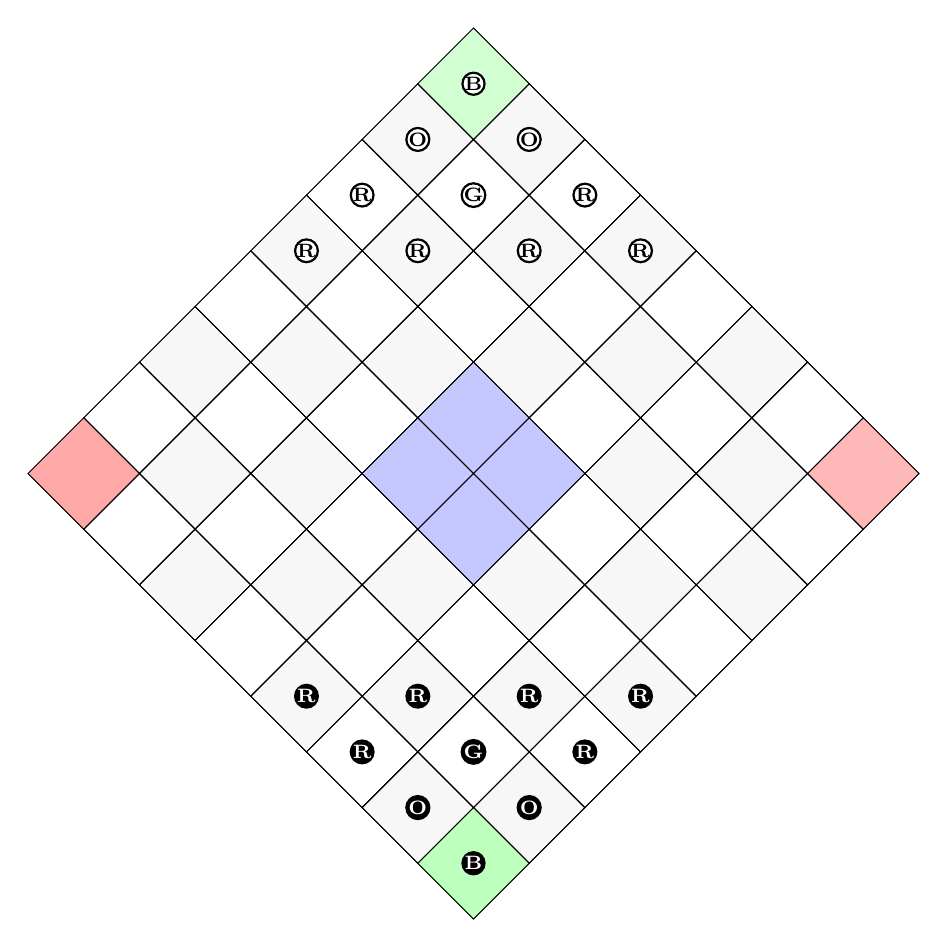
\begin{tikzpicture}[rotate=45]
  % Board + landmarks
  \DrawGrid
  \ShadeCross{cross}
  \ShadeSquares{apexA}{8/1}
  \ShadeSquares{apexB}{1/8}
  \ShadeSquares{sanctumA}{8/8}
  \ShadeSquares{sanctumB}{1/1}
  \RedrawGridLines
x
  % --- Side A (white stones) ---
  % Blue
  \PlaceA{B}{8}{1}
  % Oranges
  \PlaceA{O}{7}{1}
  \PlaceA{O}{8}{2}
  % Green
  \PlaceA{G}{7}{2}
  % Reds (R3 pair + R4 four)
  \PlaceA{R}{6}{1}
  \PlaceA{R}{8}{3}
  \PlaceA{R}{5}{1}
  \PlaceA{R}{6}{2}
  \PlaceA{R}{7}{3}
  \PlaceA{R}{8}{4}

  % --- Side B (black stones) ---
  % Blue
  \PlaceB{B}{1}{8}
  % Oranges
  \PlaceB{O}{2}{8}
  \PlaceB{O}{1}{7}
  % Green
  \PlaceB{G}{2}{7}
  % Reds (mirrored)
  \PlaceB{R}{3}{8}
  \PlaceB{R}{1}{6}
  \PlaceB{R}{4}{8}
  \PlaceB{R}{3}{7}
  \PlaceB{R}{2}{6}
  \PlaceB{R}{1}{5}
\end{tikzpicture}}
\end{subfigure}\hfill
\begin{subfigure}[t]{0.25\linewidth}
\centering
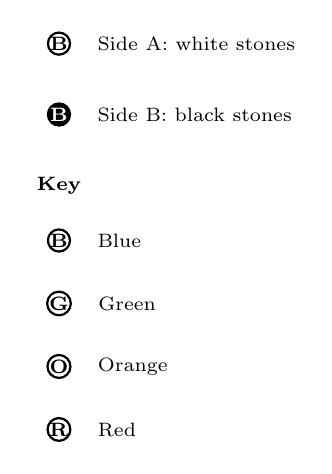
\begin{tikzpicture}
  \node[piece,fill=white] (aw) at (0,0) {\scriptsize\bfseries B};
  \node[right=6pt of aw] {\scriptsize Side A: white stones};
  \node[piece,fill=black,text=white] (bw) at (0,-0.9) {\scriptsize\bfseries B};
  \node[right=6pt of bw] {\scriptsize Side B: black stones};

  \node at (0,-1.8) {\scriptsize \bfseries Key};
  \node[piece,fill=white] (kB) at (0,-2.5) {\scriptsize\bfseries B};
  \node[right=6pt of kB] {\scriptsize Blue};
  \node[piece,fill=white] (kG) at (0,-3.3) {\scriptsize\bfseries G};
  \node[right=6pt of kG] {\scriptsize Green};
  \node[piece,fill=white] (kO) at (0,-4.1) {\scriptsize\bfseries O};
  \node[right=6pt of kO] {\scriptsize Orange};
  \node[piece,fill=white] (kR) at (0,-4.9) {\scriptsize\bfseries R};
  \node[right=6pt of kR] {\scriptsize Red};
\end{tikzpicture}
\end{subfigure}

\caption{Initial setup on the 8×8 diamond board. Circles mark stones; letters indicate type. Side A shown in white, Side B in black.}
\end{figure}
{\scriptsize\quad\textsf{A = white stones;\; B = black stones;\; B/G/O/R = Blue, Green, Orange, Red.}}

\section{Turn Order}
\label{sec:turnorder}

Players alternate turns, \textbf{one move per turn}. As opening balance, the \textbf{second player takes two moves on their first turn} (back-to-back). They \emph{may not} move the same piece twice during that opening double move. All other rules (ZoC, captures, Seed, Cross, etc.) apply normally.

\section{Basic Movement, Capture \& Zone of Control (ZoC)}
\label{sec:movement}

\subsection*{Lanes \& Directions}
Every square connects to four diagonal \textbf{lanes}: \textbf{Onward-Left (OL)} and \textbf{Onward-Right (OR)}—both toward the Opposing Apex; and \textbf{Homeward-Left (HL)} and \textbf{Homeward-Right (HR)}—both toward your Home Apex. A move travels along \emph{one} lane without turning; all intermediate squares must be empty.

\subsubsection*{Piece Movement \& Capture}
\begin{tabularx}{\linewidth}{@{}l c c l@{}}
\toprule
\textbf{Piece} & \textbf{Onward (exact)} & \textbf{Homeward (up to)} & \textbf{Capture}\\
\midrule
Red (Line)      & 2 & 1 & by displacement (move onto enemy square)\\
Orange (Officer)& 3 & 2 & by displacement\\
Green (Raider)  & 4 & 3 & by displacement\\
Blue (Royal)    & 5 & 4 & see Section \ref{sec:blue}\\
\bottomrule
\end{tabularx}

\medskip
\noindent\textbf{No passing through pieces.} You cannot move through occupied squares. A move stays on one lane (no mid-move turns).

\section*{Zone of Control (ZoC)}
Every piece exerts ZoC on the \textbf{four adjacent diagonal squares} (one step along OL, OR, HL, HR). You may \textbf{enter} an enemy ZoC square (including to capture), but \textbf{\emph{entering enemy ZoC ends your move immediately}}. You \textbf{cannot} move \emph{through} ZoC.

\subsection{Blue’s Movement \& Specials}\label{sec:blue}
Blue moves along the four lanes (OL/OR/HL/HR) as listed in the Movement table and interacts with ZoC like any piece: it may enter enemy ZoC, but any \emph{slide} ends upon entry. (ZoC does not block a \emph{legal} special.)

\paragraph{Capture specials (per Blue life).}
A Blue has two one-use capture specials, refreshed when it returns via Reforge. In any Blue turn you may use \emph{at most one} special, and you may \emph{slide then special}. After a special resolves, that Blue’s movement for the turn is over (no special$\rightarrow$slide).
\begin{enumerate}[label=(\alph*)]
  \item \textbf{Displacement} — Move one step \emph{along a lane} onto an adjacent enemy; remove it.
  \item \textbf{Hop-capture} — Jump over one adjacent enemy \emph{along the same lane} to the empty square immediately beyond; remove the jumped enemy. (Blue cannot hop without capturing.)
\end{enumerate}

\begin{tcolorbox}[enhanced,breakable,title={Rules Note — ZoC and Blue Specials}]
\small
\textbf{Legal.} Blue may use \emph{hop-capture} or \emph{displacement} even if the \emph{landing square} lies inside enemy ZoC; captures end the move. Blue may also begin its turn standing in ZoC and use a special from there.

\textbf{Not legal.} You may \emph{not} slide into enemy ZoC and then use a special on the same turn: entering ZoC by sliding immediately ends the move.

\textit{Example.} From adjacency, Blue may hop over an enemy into an empty square that is in ZoC. But “slide one step into ZoC to become adjacent, then hop” is illegal.
\end{tcolorbox}

\paragraph{Crown Stagger (core).}
When your Blue uses its \emph{second} capture special in the same Blue life (one Hop and one Displacement, in any order), then at the \textbf{end of that turn} your Blue becomes \textbf{Rooted} until your \textbf{next turn begins}. It still exerts ZoC and may be captured. Blue never promotes.

\section{Twin Apex Seed (Spawning Greens)}
\label{sec:twinapex}
If your Blue \textbf{ends its move on a Sanctum}, you may \textbf{spawn one Green on the opposite Sanctum} (if empty and the Global Green Cap is not exceeded). After seeding, that Blue becomes \textbf{Rooted} (it may not move) until \textbf{your next turn begins}.\\[2pt]
\paragraph{Mobilization Seed-Delay (scope).}
On the \emph{first turn that a given Blue leaves its Home Apex for that Blue’s current life}, you \textbf{cannot} use Twin Apex Seed, even if it ends that move on a Sanctum. 
This restriction \textbf{resets each time that Blue returns via Reforge} (i.e., each new Blue life).

\begin{tcolorbox}[enhanced,breakable,title={Rules Note — Mobilization Delay \& Reforge→Sanctum Seeding},
  colback=white,colframe=royal,boxrule=0.8pt]
\small
\textbf{Mobilization delay.} A Blue may \emph{not} Seed on that Blue’s \emph{first departure from Home} in its current life.
(Being placed on a Sanctum by Reforge is \emph{not} a departure.)

\medskip
\textbf{Reforge→Sanctum, then Seed from the opposite (allowed).} A Blue placed by Reforge on \emph{Sanctum A}
may later end a turn on \emph{Sanctum B} and \textbf{Seed}, spawning the Green on \emph{Sanctum A}, without ever
visiting Home, provided:
\begin{itemize}[leftmargin=1.1em,itemsep=0.2em]
  \item the opposite Sanctum is empty;
  \item the global Green cap is $<6$;
  \item the Blue is not \textbf{Rooted}.
\end{itemize}
The \textbf{same-Sanctum ban} forbids Seeding only from the exact Sanctum used for the Reforge placement;
\textbf{Mobilization delay} applies only on the Blue’s first departure from \emph{Home} in that life.
\end{tcolorbox}


\section{Central Four (the “Cross”)}
\label{sec:bluecross}

The \textbf{Cross} is the 2×2 diamond of squares at board center. Only Blue has special timing there:
\begin{itemize}
  \item A Blue may enter and occupy the Cross normally.
  \item \textbf{Stay limit:} A given Blue may remain in the Cross for at most \textbf{3 of its own turns} (not counting the opponent’s turns). Exceeding this is illegal; the Blue must exit before its fourth turn in the Cross.
  \item \textbf{Exclusion on exit:} After a Blue leaves the Cross, it \textbf{cannot re-enter the Cross for the next 2 of its turns}.
\end{itemize}

\noindent\emph{Illegal CF end (a fourth stay) is rewound to the start of that move; choose a legal move. Tournament penalties, see \ref{sec:tournament-options}.}

\begin{tcolorbox}[enhanced,breakable,title={Rules Note — Cross Timers \& the Opening Double-Move},
  colback=white,colframe=royal,boxrule=0.8pt]
\small
\textbf{No opening interaction.} From the normal setup, neither side can enter the Central Four on their first turn; P2’s double-move does not affect Cross counters.

\textbf{Stays \& Exclusion (general).}
\begin{itemize}[leftmargin=1.1em,itemsep=0.2em]
  \item \textbf{Stay} increases only if your \emph{turn ends} with your Blue on a Cross square.
  \item \textbf{Exclusion} begins only when that same Blue later \emph{leaves} the Cross after a counted stay.
  \item Example timeline: Turn \(N\): Blue enters \(\Rightarrow\) \([{\tt CF:in~1/3}]\). Turn \(N{+}1\): still inside \(\Rightarrow\) \([{\tt in~2/3}]\). Turn \(N{+}2\): exits \(\Rightarrow\) \([{\tt ex~1/2}]\). Turn \(N{+}3\): \([{\tt ex~2/2}]\). Turn \(N{+}4\): re-entry allowed.
\end{itemize}
\end{tcolorbox}

\noindent\begin{tabularx}{\linewidth}{@{}l X@{}}
\toprule
\textbf{Central Four (“Cross”) — Summary} & \textbf{Effect}\\
\midrule
Enter Cross & Legal; normal ZoC applies.\\
Stay timer & Max \textbf{3 of that Blue’s turns} inside.\\
Exit & Must leave before its \textbf{4th} own turn while in-Cross.\\
Re-entry & Excluded for the next \textbf{2 of that Blue’s turns}.\\
\bottomrule
\end{tabularx}

\section{Reforge (Blue Return After Capture)}\label{sec:reforge}
When your Blue is captured, a \textbf{five-turn countdown} begins: you have \textbf{5 of your own turns} to \textbf{plant a banner} by \textbf{occupying the enemy Home Apex} with any one of your pieces. If you fail, you \textbf{lose immediately}.

\subsection*{Plant \textrightarrow\ Remove Runner \textrightarrow\ Return Blue (choose placement & pay cost)}
On the turn you occupy the enemy Home Apex:
\begin{enumerate}
  \item \textbf{Plant the banner:} End your move on the enemy Home Apex.
  \item \textbf{Remove the runner:} The occupying piece leaves play (remove it).
  \item \textbf{Place your Blue:} Choose \emph{one} of:
  \begin{itemize}
     \item \textbf{Opposing Apex} — sacrifice one of your Greens (the runner may pay).
     \item \textbf{Either Sanctum} — that Blue may never Seed from that same Sanctum later.
  \item \textbf{Your Home Apex} — no cost.
  \end{itemize}
  \item \textbf{Blue refresh:} A reforged Blue returns with \textbf{both capture specials unused} (fresh life).
\end{enumerate}



\section{Quick Reference}
\label{sec:quickreference}


\section*{Movement \& Capture (summary)}
\begin{tabularx}{\linewidth}{@{}l c c l@{}}
\toprule
\textbf{Piece} & \textbf{Onward (exact)} & \textbf{Homeward (up to)} & \textbf{Capture}\\
\midrule
Red    & 2 & 1 & displacement\\
Orange & 3 & 2 & displacement\\
Green  & 4 & 3 & displacement\\
Blue   & 5 & 4 & specials only (see below)\\
\bottomrule
\end{tabularx}

\noindent\footnotesize\textit{Key:} %
\On[OL]{k}/\Hm[HR]{k} = lane-tagged slides; %
\SC{H}/\SC{D} = Blue specials; %
\CC{in 1/3} = Cross timer; %
\RoC = Rooted; %
\RC = Reforge; %
\CapC{2--1} = Greens on board.\normalsize

\paragraph{Lane-tagged slides.}
Whenever a rule or example specifies a slide, we may write the lane explicitly: \(\On[\mathrm{OL}]{k}\), \(\On[\mathrm{OR}]{k}\), \(\Hm[\mathrm{HL}]{k}\), \(\Hm[\mathrm{HR}]{k}\). These tags name the exact Onward/Homeward lane used. Blue specials (\emph{Hop}, \emph{Displacement}) are annotated separately and are not written with step counts.

\section*{Notation (Lanes and Steps)}
\begin{quote}\small
Squares are indexed by \emph{lanes} $(o,h)$: your \textbf{Onward} lane $o$ (toward the opponent’s apex) and your
\textbf{Homeward} lane $h$ (toward your own apex). We write moves with lane tags:
\end{quote}

\begin{tabularx}{\linewidth}{@{}l >{\raggedright\arraybackslash}X@{}}
\textbf{Lane tags} &
\texttt{OL}=Onward-Left,\ \texttt{OR}=Onward-Right,\ \texttt{HL}=Homeward-Left,\ \texttt{HR}=Homeward-Right.\\

\textbf{Slides} &
\On[OL]{2} means slide two steps along your OL lane; \Hm[HR]{1} one step along HR.\\

\textbf{Un-tagged} &
If a tag is omitted (e.g., \On{2}), the intended lane is clear from diagram or context.\\

\textbf{Specials} &
A:\ \SC{H}\ (Hop used);\ B:\ \SC{D}\ (Displacement used).\\

\textbf{Timers} &
\CC{in 1/3}/\CC{ex 1/2}\ = Cross counters;\ \RoC{} = Rooted;\ \RC{} = Reforge;\ \CapC{2--1} = Greens on board (A–B).\\
\end{tabularx}

Lane tags are board-standard on the diamond: “left/right” are relative to your Onward/Homeward facing, not compass points.
\end{quote}

\subsection*{ZoC (summary)}
Each piece projects ZoC to the four \textbf{diagonal-adjacent} squares (one step along OL, OR, HL, HR). \textbf{Entering ZoC ends your move.}

\subsection*{Blue Specials (summary)}
\begin{itemize}
  \item \textbf{One special max per Blue turn.} May \textbf{slide, then use one} special.
  \item \textbf{Displacement (×1/life):} Step \emph{one square along the current lane} onto an adjacent enemy; remove it.
  \item \textbf{Hop (×1/life):} Jump \emph{over one adjacent enemy along the same lane} to the empty square immediately beyond; remove the jumped enemy.
  \item \textbf{Movement + special: Blue may slide and then use one special unless the slide entered enemy ZoC.}
\end{itemize}

\subsection*{Twin Apex Seed (summary)}
End Blue’s move on a Sanctum $\rightarrow$ spawn a Green on the opposite Sanctum (if empty, cap OK) $\rightarrow$ that Blue is \textbf{Rooted} until your next turn. \textbf{Cannot} Seed on Blue’s \emph{first} departure from Home Apex.

\subsection*{Central Four (“Cross”) (summary)}
Max \textbf{3 of that Blue’s turns} inside; after exiting, \textbf{cannot re-enter for 2 of its turns}.

\noindent\textbf{Violations.} Rewind to the last legal position before the illegal end-of-turn and enforce a legal move.

\subsection*{Reforge (summary)}
\begin{enumerate}
  \item Capture Blue $\rightarrow$ defender gets \textbf{5 of their turns} to plant a banner (occupy enemy Home Apex).
  \item On plant: \textbf{remove runner} $\rightarrow$ \textbf{place Blue} at Opposing Apex (sacrifice a Green), \emph{or} either Sanctum (no Seed from that Sanctum for this life), \emph{or} Home Apex (free).
  \item Blue returns with \textbf{both specials unused}.
\end{enumerate}

\subsection*{Timing Notes}
\begin{itemize}
  \item The five-turn count advances after each of \emph{your} turns.
  \item If the capture occurs during the second player’s opening double-move, the defender still receives a full five of their turns thereafter.
\end{itemize}

\textbf{Win:} Opponent fails Reforge after you capture their Blue.\\
\textbf{Draws} (by agreement or adjudication):
\begin{itemize}
  \item \textbf{Stalemate/mutual blockade:} No legal progress toward Blue capture or banner plant is reasonably possible for either side. Organizers may apply a move-count rule (e.g., 50 full turns without a capture or Seed).
  \item \textbf{Threefold repetition:} The same position (including all timers/flags/counters) with the same player to move occurs three times. See \nameref{sec:tournament-options}
\end{itemize}
\textbf{Concession} ends the game immediately.

\section{Illegal Moves \& Clarifications}
\label{sec:clarifications}

\begin{itemize}
  \item Moves travel along a single \textbf{lane} (OL/OR toward Opposing Apex; HL/HR toward Home Apex) with no mid-move turns; \textbf{no passing through pieces}.
  \item You \textbf{cannot} move through enemy ZoC; you \textbf{may} \emph{enter} ZoC (including to capture), but \textbf{entering enemy ZoC ends your move}.
  \item Only \textbf{Blue} can hop, and only as a \textbf{hop-capture along its current lane}.
  \item You \textbf{cannot} Seed if the opposite Sanctum is occupied or doing so would exceed the Global Green Cap.
  \item The Reforge runner may be \emph{any} of your pieces.
  \item Blue may \textbf{slide then use} one special (if legal); it may \textbf{not} use both specials in the same turn.
\end{itemize}

\section{Table Etiquette (recommended)}
\label{sec:etiquette}


Keep a \textbf{five-turn counter} for Reforge, \textbf{two markers} to track Blue’s specials, and \textbf{six beads} for the global Green cap. Announce “\textit{Seed}” and “\textit{Reforge}” aloud to avoid ambiguity. When in doubt, replay from the last clear position.

\vfill
\hrule
\small
\textit{Kon'reh rewards clarity. Forward is commitment; sideways is breath. Seed for tomorrow; map your Reforge today.}
\clearpage

% Flush earlier floats so they don't push this figure away
\FloatBarrier
% If there isn't room for heading+figure together, start a fresh page now
\needspace{0.80\textheight}


\section{Board Diagrams \& Core Concepts}
\vspace{-0.4\baselineskip}

% ==== ONE-PAGE LAYOUT: Board + ZoC + Movement ====
\begin{figure}[H] % force here to keep with section header
\centering
\captionsetup{aboveskip=0.5ex,belowskip=0.4ex}
\captionsetup[sub]{font=small,labelfont=bf,justification=centering}

% -------- Top: full board (fits width) --------
\begin{subfigure}[t]{0.90\linewidth}
\centering
\resizebox{0.68\linewidth}{!}{%
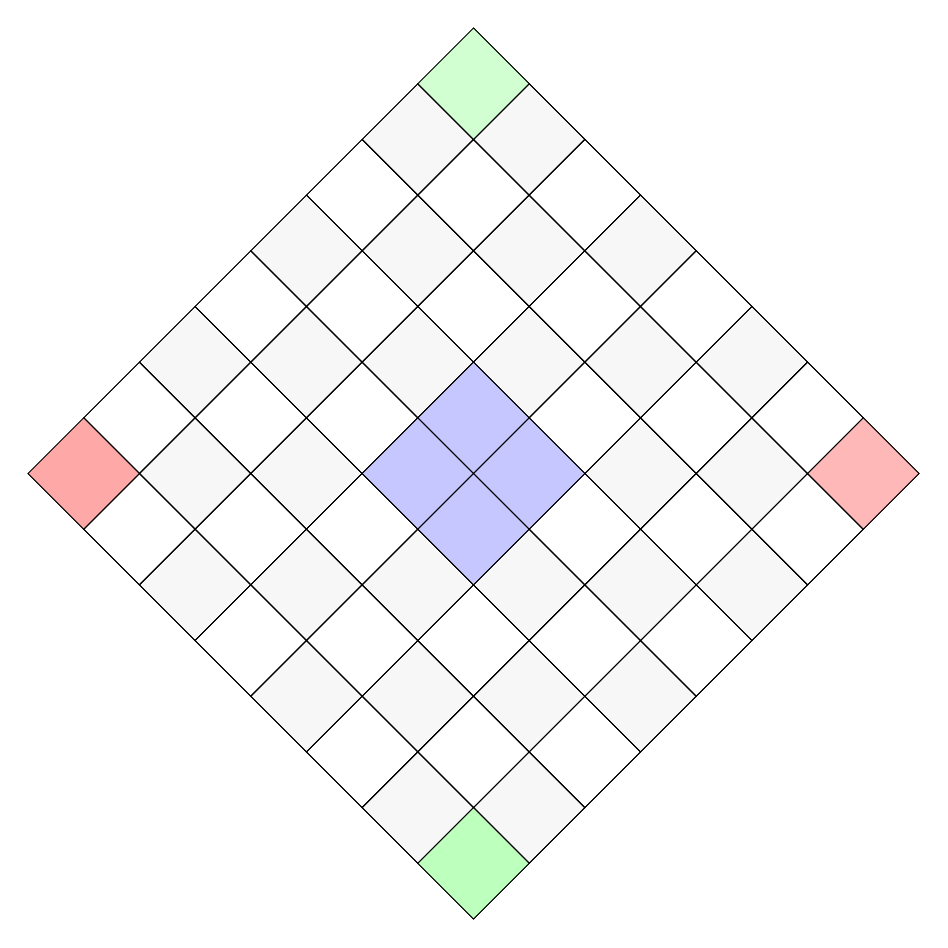
\begin{tikzpicture}[rotate=45]
  % Base board
  \DrawGrid
  % Central Four (blue)
  \ShadeCross{cross}
  % Home apex squares (green) — post-rotate "top" and "bottom"
  \ShadeSquares{apexA}{8/1}
  \ShadeSquares{apexB}{1/8}
  % Sanctums (red) — side apex squares
  \ShadeSquares{sanctumA}{8/8}
  \ShadeSquares{sanctumB}{1/1}
  % Grid outlines back on top
  \RedrawGridLines
\end{tikzpicture}}
\caption{Diamond board (8×8) with the \emph{Central Four} (blue), Home apex squares (green), and side-apex \emph{Sanctums} (red).}
\end{subfigure}

\vspace{0.4em}

% -------- Bottom: two minis side-by-side --------
\begin{subfigure}[t]{0.47\linewidth}
\centering
\resizebox{\linewidth}{!}{%
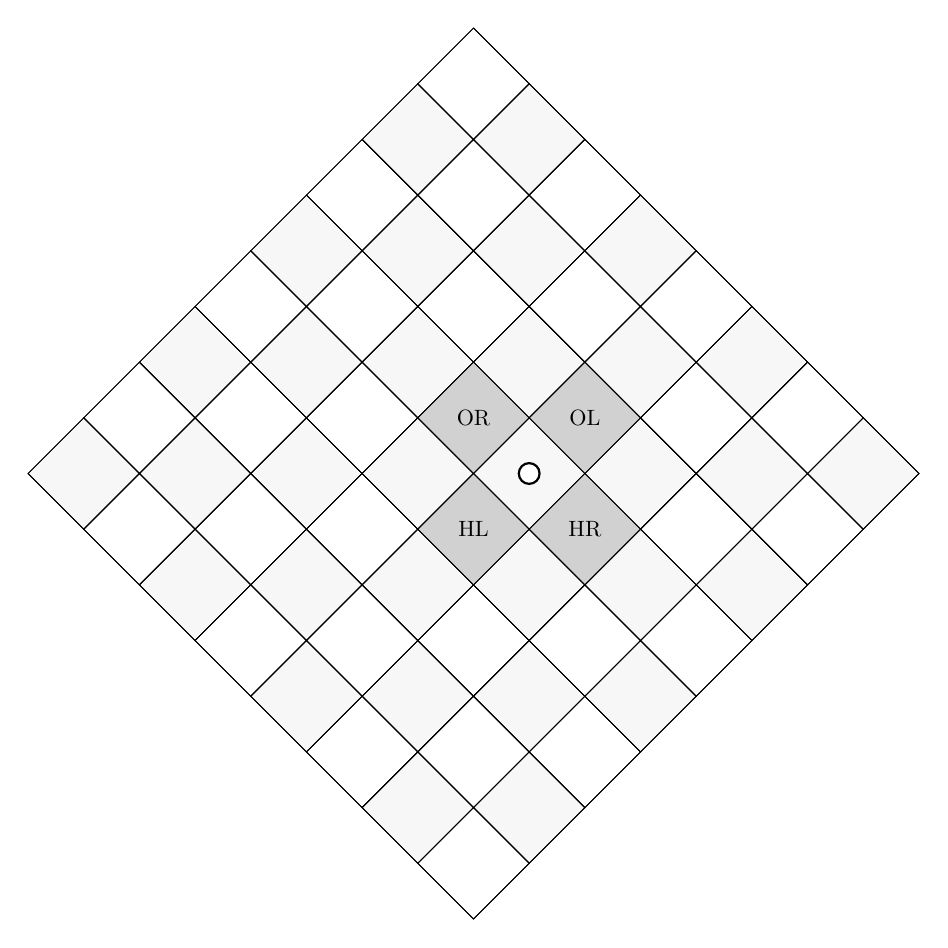
\begin{tikzpicture}[rotate=45]
  \DrawGrid
  % Center piece
  \def\cx{5}\def\cy{5}
  \pgfmathtruncatemacro{\yP}{\BoardN-\cy}
  \node[piece] (P) at ({\cx-0.5},{\yP+0.5}) {};
  % Cardinal ZoC (HL/HR/OL/OR)
  \foreach \dx/\dy/\lab in {-1/0/\LabelW, 1/0/\LabelE, 0/-1/\LabelN, 0/1/\LabelS}{%
    \pgfmathtruncatemacro{\nx}{\cx+\dx}%
    \pgfmathtruncatemacro{\ny}{\cy+\dy}%
    \ifnum\nx>0\relax\ifnum\nx<\numexpr\BoardN+1\relax
    \ifnum\ny>0\relax\ifnum\ny<\numexpr\BoardN+1\relax
      \pgfmathtruncatemacro{\yphys}{\BoardN-\ny}%
      \path[zoc] ({\nx-1},{\yphys}) rectangle ++(1,1);
      \node[scale=0.8] at ({\nx-0.5},{\yphys+0.5}) {\lab};
    \fi\fi\fi\fi
  }
  \RedrawGridLines
\end{tikzpicture}}
\caption{Zone of Control: the four \emph{cardinal} neighbors (HL/HR/OL/OR).}
\end{subfigure}\hfill
\begin{subfigure}[t]{0.47\linewidth}
\centering
\resizebox{\linewidth}{!}{%
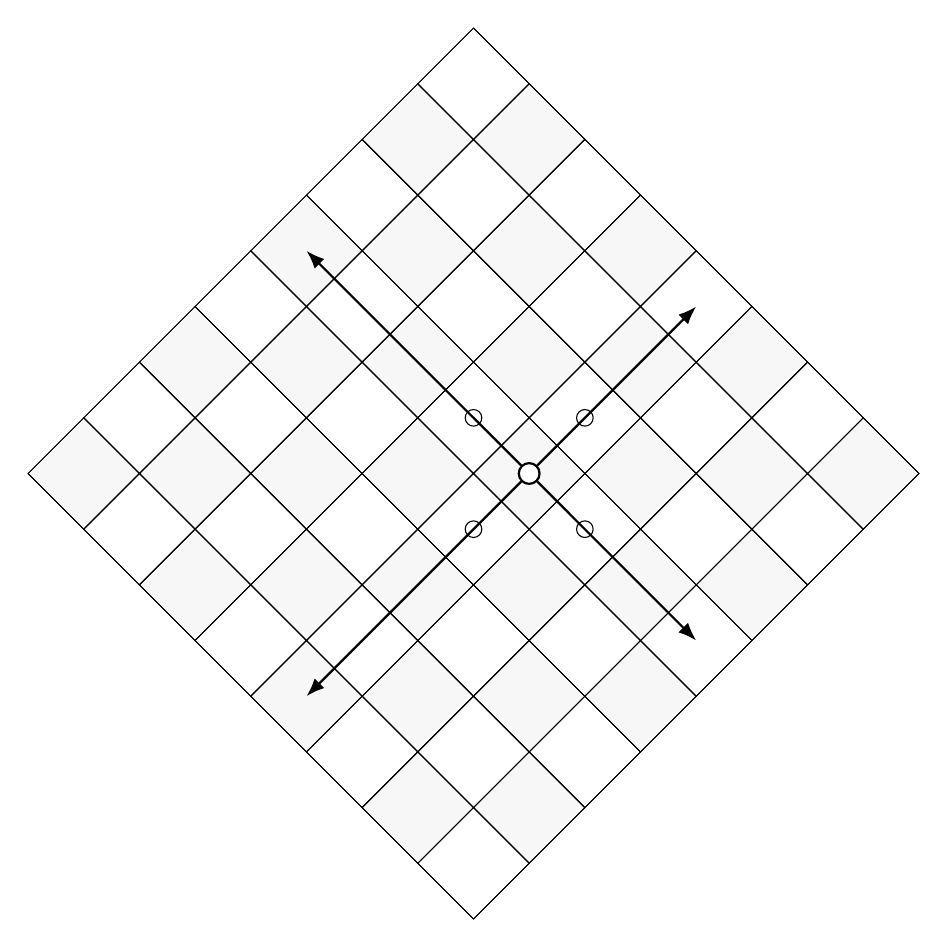
\begin{tikzpicture}[rotate=45]
  \DrawGrid
  % Same start square
  \def\cx{5}\def\cy{5}
  \pgfmathtruncatemacro{\yQ}{\BoardN-\cy}
  \node[piece] (Q) at ({\cx-0.5},{\yQ+0.5}) {};
  % Cardinal movement lanes (no ZoC shading)
  \draw[moveArrow] (Q) -- ({\BoardN-0.5},{\yQ+0.5}); % east
  \draw[moveArrow] (Q) -- ({0.5},{\yQ+0.5});         % west
  \draw[moveArrow] (Q) -- ({\cx-0.5},{0.5});         % south
  \draw[moveArrow] (Q) -- ({\cx-0.5},{\BoardN-0.5}); % north
  % One-step target markers for steppers
  \foreach \dx/\dy in {-1/0,1/0,0/-1,0/1}{%
    \pgfmathtruncatemacro{\tx}{\cx+\dx}%
    \pgfmathtruncatemacro{\ty}{\cy+\dy}%
    \ifnum\tx>0\relax\ifnum\tx<\numexpr\BoardN+1\relax
    \ifnum\ty>0\relax\ifnum\ty<\numexpr\BoardN+1\relax
      \pgfmathtruncatemacro{\yT}{\BoardN-\ty}%
      \node[draw,circle,minimum size=6pt,inner sep=0pt] at ({\tx-0.5},{\yT+0.5}) {};
    \fi\fi\fi\fi
  }
  \RedrawGridLines
\end{tikzpicture}}
\caption{Movement lanes are \emph{cardinal} on the diamond board (HL/HR/OL/OR).}
\end{subfigure}

\caption{Board overview with \emph{Central Four}, cardinal ZoC, and cardinal movement lanes.}
\end{figure}
% ==============================
% PAGE 2: Lane legend + notation
% ==============================
\begin{figure}[p]
\centering

% ---- (A) Lane legend: two through-lanes through a square ----
\begin{subfigure}[t]{0.48\linewidth}
\centering
\resizebox{\linewidth}{!}{%
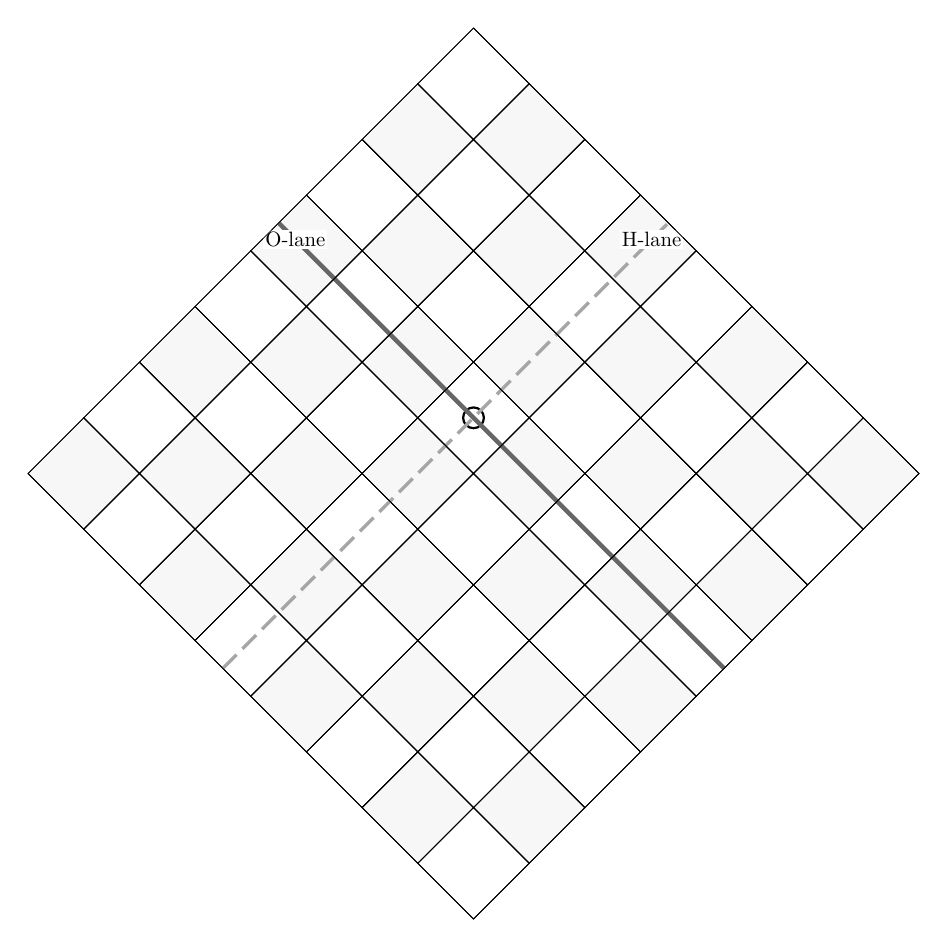
\begin{tikzpicture}[rotate=45]
  \DrawGrid
  % focus square (choose any of the four Cross squares)
  \def\cx{5}\def\cy{4}
  \pgfmathtruncatemacro{\yy}{\BoardN-\cy}
  % piece at focus
  \node[piece] (C) at ({\cx-0.5},{\yy+0.5}) {};
  % lane styles (local)
  \tikzset{laneO/.style={line width=1.6pt, draw=black!60},
           laneH/.style={line width=1.2pt, draw=black!35, dash pattern=on 7pt off 3pt}}
  % O-lane (vertical through-lane through square center)
  \draw[laneO] ({\cx-0.5},0) -- ({\cx-0.5},\BoardN);
  % H-lane (horizontal through-lane through square center)
  \draw[laneH] (0,{\yy+0.5}) -- (\BoardN,{\yy+0.5});
  % subtle lane labels
  \node[scale=0.75, fill=white, inner sep=1pt] at ({\cx-0.5},\BoardN-0.3) {O-lane};
  \node[scale=0.75, fill=white, inner sep=1pt] at (\BoardN-0.3,{\yy+0.5}) {H-lane};
  \RedrawGridLines
\end{tikzpicture}}
\caption{Every square lies at the intersection of two through-lanes: one O-lane and one H-lane.}
\end{subfigure}\hfill
% ---- (B) Notation key: (o,h) coordinates on lanes ----
\begin{subfigure}[t]{0.48\linewidth}
\centering
\resizebox{\linewidth}{!}{%
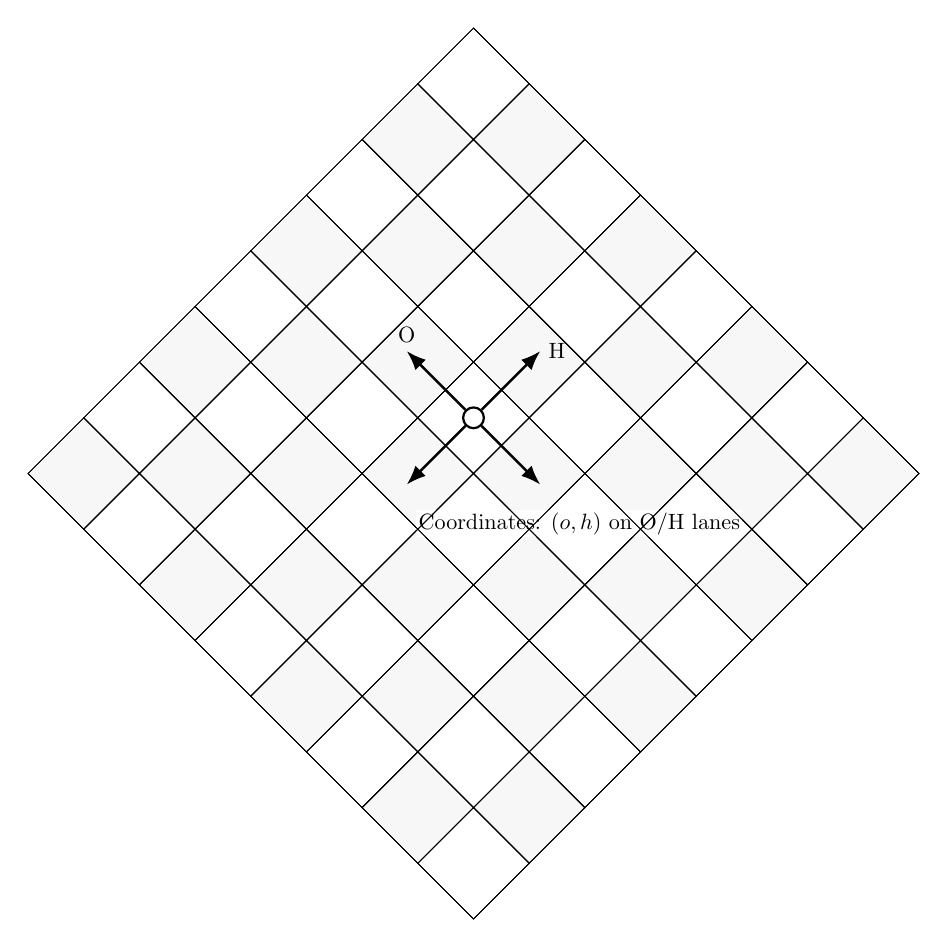
\begin{tikzpicture}[rotate=45]
  \DrawGrid
  % focus square
  \def\cx{5}\def\cy{4}
  \pgfmathtruncatemacro{\yy}{\BoardN-\cy}
  \node[piece] (C) at ({\cx-0.5},{\yy+0.5}) {};
  % short arrows indicating lane directions from the square
  \draw[-Latex, line width=0.9pt] (C) -- ++(0,1.2) node[above,scale=0.8]{O};
  \draw[-Latex, line width=0.9pt] (C) -- ++(0,-1.2);
  \draw[-Latex, line width=0.9pt] (C) -- ++(1.2,0) node[right,scale=0.8]{H};
  \draw[-Latex, line width=0.9pt] (C) -- ++(-1.2,0);
  % coordinate label
  \node[scale=0.8, fill=white, inner sep=1pt] at ($(C)+(0.0,-1.9)$) {Coordinates: $(o,h)$ on O/H lanes};
  \RedrawGridLines
\end{tikzpicture}}
\caption{Notation: index squares by their O- and H-lane coordinates \((o,h)\).
\(o\) increases along the Onward lane (toward the opposing apex); \(h\) increases along the orthogonal Homeward lane.}
\end{subfigure}

\caption{Lane legend and notation. O/H are the two canonical through-lanes used for movement and control.}
\end{figure}

% ==============================
% PAGE 3: Capture vs. block (lane runners)
% ==============================
\begin{figure}[p]
\centering

% ---- (A) Friendly block: stop one before ----
\begin{subfigure}[t]{0.48\linewidth}
\centering
\resizebox{\linewidth}{!}{%
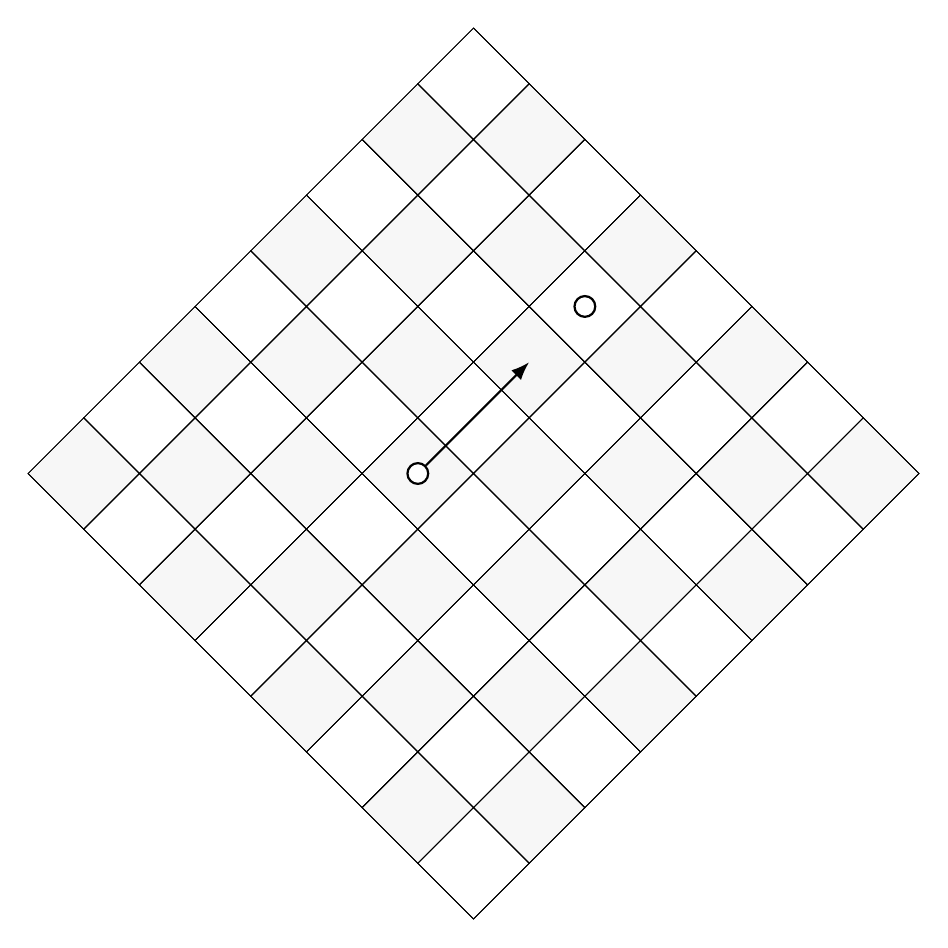
\begin{tikzpicture}[rotate=45]
  \DrawGrid
  % start piece
  \def\cx{4}\def\cy{4}
  \pgfmathtruncatemacro{\yy}{\BoardN-\cy}
  \node[piece] (S) at ({\cx-0.5},{\yy+0.5}) {};
  % friendly blocker to the right on same H-lane
  \def\fx{7}\def\fy{4}
  \pgfmathtruncatemacro{\fyphys}{\BoardN-\fy}
  \node[piece] (F) at ({\fx-0.5},{\fyphys+0.5}) {};
  % arrow stops one before the friendly
  \draw[moveArrow] (S) -- ({\fx-1-0.5},{\fyphys+0.5});
  \RedrawGridLines
\end{tikzpicture}}
\caption{Friendly piece on the lane: the run stops one square before.}
\end{subfigure}\hfill
% ---- (B) Enemy block: capture on contact ----
\begin{subfigure}[t]{0.48\linewidth}
\centering
\resizebox{\linewidth}{!}{%
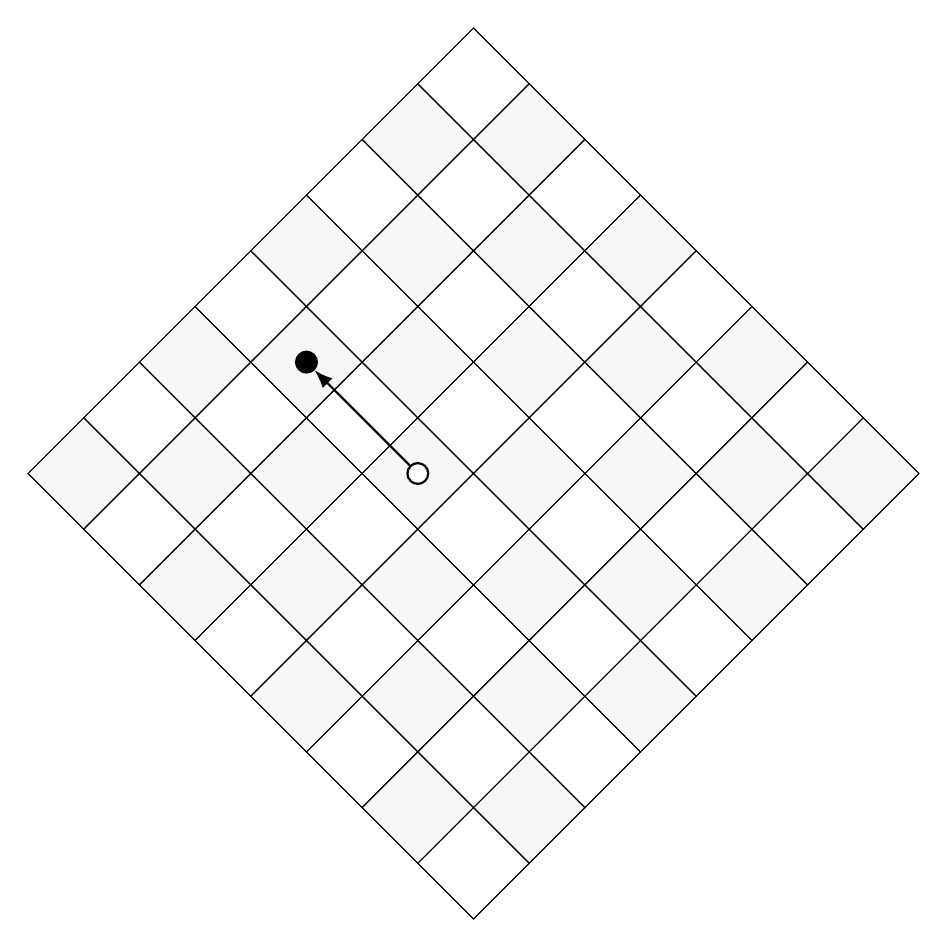
\begin{tikzpicture}[rotate=45]
  \DrawGrid
  % start piece
  \def\cx{4}\def\cy{4}
  \pgfmathtruncatemacro{\yy}{\BoardN-\cy}
  \node[piece] (S) at ({\cx-0.5},{\yy+0.5}) {};
  % enemy blocker ahead on O-lane (downward from viewer)
  \def\ex{4}\def\ey{2}
  \pgfmathtruncatemacro{\eyphys}{\BoardN-\ey}
  \node[piece, fill=black] (E) at ({\ex-0.5},{\eyphys+0.5}) {};
  % arrow terminates on the enemy square (capture)
  \draw[moveArrow] (S) -- (E);
  \RedrawGridLines
\end{tikzpicture}}
\caption{Opposing piece on the lane: the run terminates on that square (capture).}
\end{subfigure}

\caption{Lane runners interacting with pieces ahead: friendly blocks vs. opposing captures.}
\end{figure}

% ==============================
% PAGE 4: Edge & corner behavior
% ==============================
\begin{figure}[p]
\centering

% ---- (A) Edge example: lanes truncated ----
\begin{subfigure}[t]{0.48\linewidth}
\centering
\resizebox{\linewidth}{!}{%
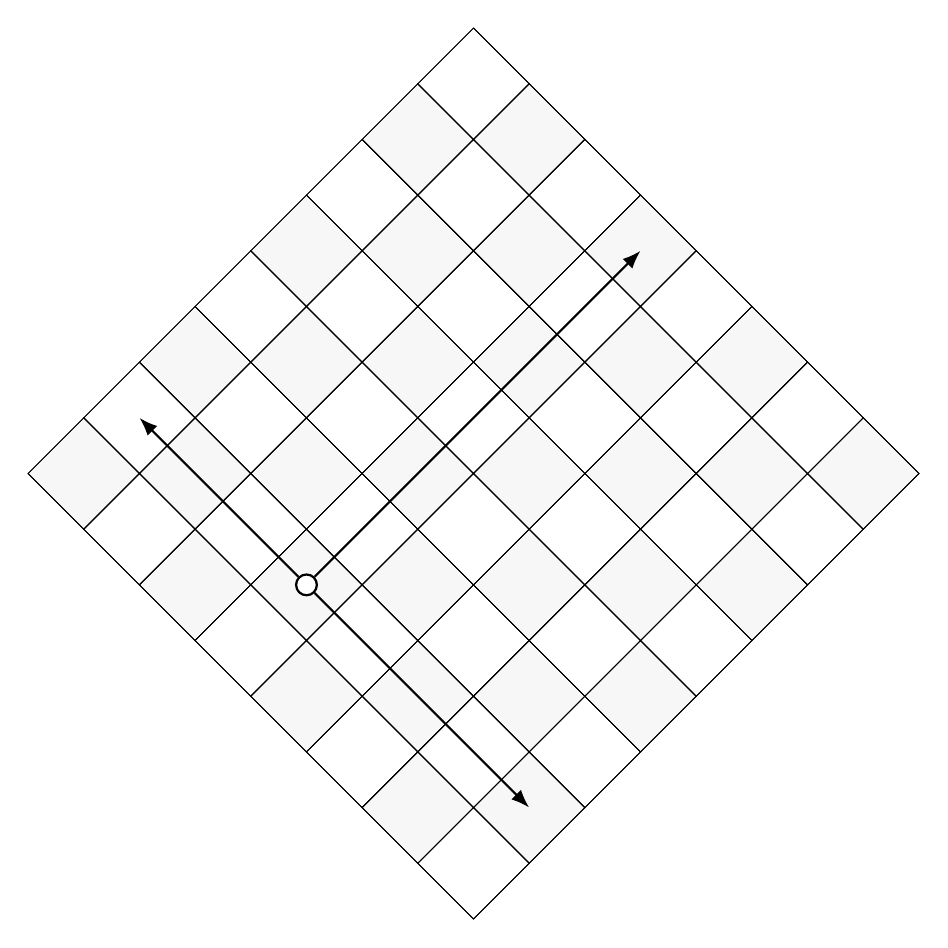
\begin{tikzpicture}[rotate=45]
  \DrawGrid
  % place piece near the left edge on Cross rank
  \def\cx{2}\def\cy{4}
  \pgfmathtruncatemacro{\yy}{\BoardN-\cy}
  \node[piece] (E) at ({\cx-0.5},{\yy+0.5}) {};
  % available runs along O/H lanes from edge position
  \draw[moveArrow] (E) -- ({\BoardN-0.5},{\yy+0.5}); % across
  \draw[moveArrow] (E) -- ({\cx-0.5},{0.5});         % downward
  \draw[moveArrow] (E) -- ({\cx-0.5},{\BoardN-0.5}); % upward
  \RedrawGridLines
\end{tikzpicture}}
\caption{On an edge, one side of a lane is already gone; runs only extend where squares exist.}
\end{subfigure}\hfill
% ---- (B) Corner example: lanes minimal ----
\begin{subfigure}[t]{0.48\linewidth}
\centering
\resizebox{\linewidth}{!}{%

\begin{tikzpicture}[rotate=45]
  \DrawGrid
  % corner piece (use a side-apex to demonstrate)
  \def\cx{1}\def\cy{1}
  \pgfmathtruncatemacro{\yy}{\BoardN-\cy}
  \node[piece] (C) at ({\cx-0.5},{\yy+0.5}) {};
  % only two runs are possible from a corner
  \draw[moveArrow] (C) -- ({\BoardN-0.5},{\yy+0.5}); % across
  \draw[moveArrow] (C) -- ({\cx-0.5},{\BoardN-0.5}); % upward
  \RedrawGridLines
\end{tikzpicture}}
\caption{In a corner, lanes reduce to the two that remain.}
\end{subfigure}

\caption{Reduced options at the edge and corner.}
\end{figure}

% ==============================
% PAGE 5: Sanctum interaction (enter & bank)
% ==============================
\begin{figure}[p]
\centering

% ---- (A) Entering a side-apex Sanctum ----
\begin{subfigure}[t]{0.48\linewidth}
\centering
\resizebox{\linewidth}{!}{%
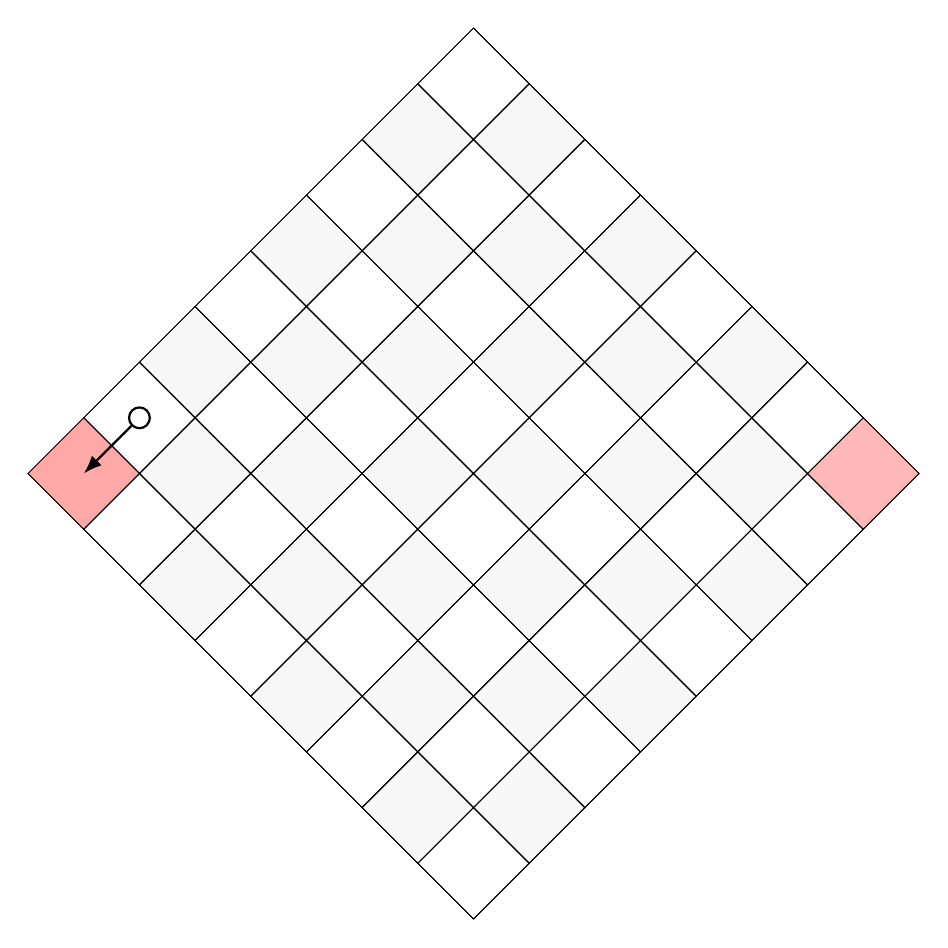
\begin{tikzpicture}[rotate=45]
  \DrawGrid
  % highlight sanctums (optional)
  \ShadeSquares{sanctumA}{8/8}
  \ShadeSquares{sanctumB}{1/1}
  \RedrawGridLines
  % approach from adjacent H-lane square toward the left sanctum (1/1)
  \def\sx{2}\def\sy{1}
  \pgfmathtruncatemacro{\yy}{\BoardN-\sy}
  \node[piece] (S) at ({\sx-0.5},{\yy+0.5}) {};
  \draw[moveArrow] (S) -- ({1-0.5},{\yy+0.5});
\end{tikzpicture}}
\caption{Entering a side-apex Sanctum along a lane.}
\end{subfigure}\hfill
% ---- (B) Banking a reserve on Sanctum ----
\begin{subfigure}[t]{0.48\linewidth}
\centering
\resizebox{\linewidth}{!}{%
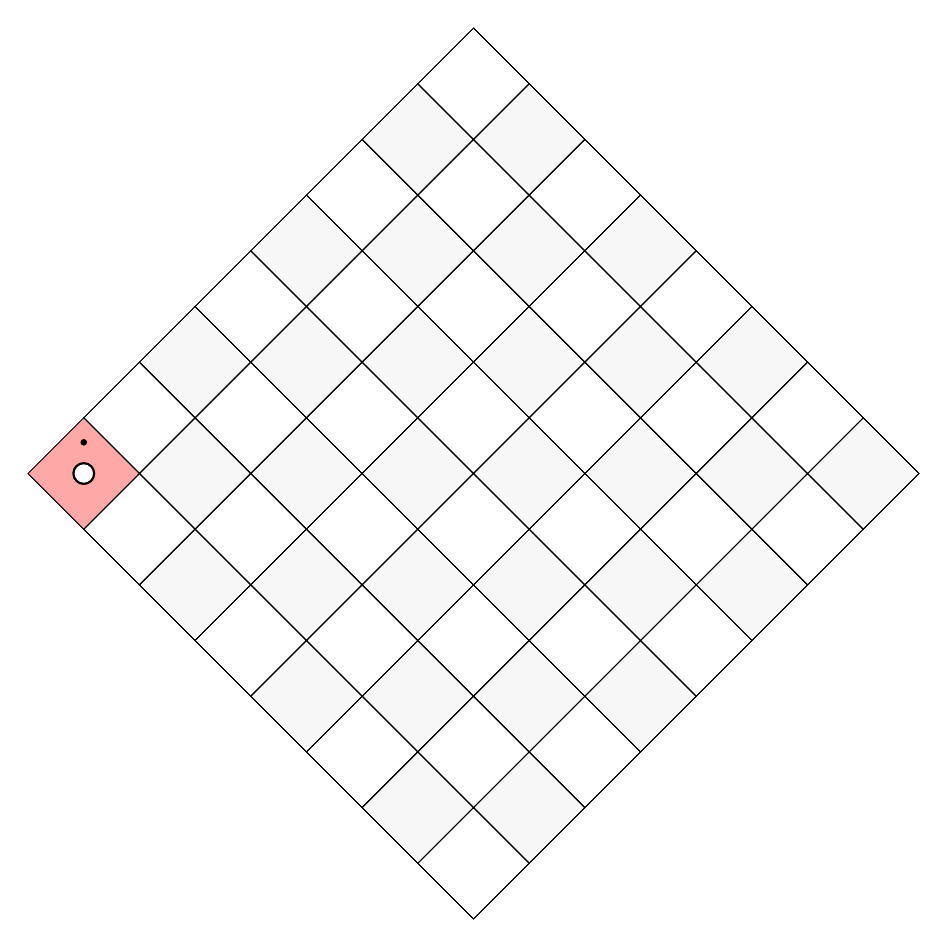
\begin{tikzpicture}[rotate=45]
  \DrawGrid
  % show piece resting on sanctum and a small "pip"
  \def\cx{1}\def\cy{1}
  \pgfmathtruncatemacro{\yy}{\BoardN-\cy}
  \ShadeSquares{sanctumB}{1/1}
  \RedrawGridLines
  \node[piece] (P) at ({\cx-0.5},{\yy+0.5}) {};
  % tiny parity pip near the piece
  \fill ( {(\cx-0.5)+0.28} , {(\yy+0.5)+0.28} ) circle (1.2pt);
\end{tikzpicture}}
\caption{Waiting on a Sanctum may bank a reserve, by table rule.}
\end{subfigure}

\caption{Sanctums at the side apex squares: entering and holding.}
\end{figure}


\clearpage
\section{Strategy \& Training Guide}
\label{sec:guide}

% === just after \section{Strategy \& Training Guide} ===
\vspace{-0.5em}
\begin{quote}\small
\textit{“I watched an Oshiiran marshal play not for squares but for \emph{throughput}. He hung two lanterns on the market’s edge and called them exits; the crowd did not see the lamps were \emph{certificates}\footnote{The translator glosses Safiya’s ‘lanterns’ as the Oshiiran practice of proving \emph{two certain exits} before a central incursion; cf.\ our XS (\emph{Exit Certainty}).}. When his Blue stepped into the desert, he drank once, twice, thrice—and never a fourth\footnote{Safiya’s ‘desert’ is the central four. Her ‘three drinks’ aligns with the Cross stay limit of three turns.}. The merchants with drums called this caution. It was geometry.}

\textit{He did not harvest material; he priced routes. The first Orange set the levy where feet must fall, the Reds laid bridges \emph{not} to cross but to \emph{close} behind. When a Sanctum answered, his captain rooted himself like a quartermaster with both hands on the ledger\footnote{Safiya’s image of the ‘rooted quartermaster’ foreshadows the modern \emph{Rooted} state after Seed and the Crown Stagger consequence of spending both Blue captures in a single life.}, and from the opposite quay a Green packet slid out with the tide.}

\textit{You will say this is slow. It is only quiet. See how the five dawns were counted before the first strike: a depot planted far; a lane welded late; a Cross touched and left with dignity; a runner shown and then priced away; the banner race forced to end on a bookkeeper’s page. The victory was not a blow but a balance: when every profitable road belonged to him, the other player resigned like a caravan turning at a toll.”}
\end{quote}
\begin{flushright}\small
— rendered by \textit{Aqyl of Thypergos}, fol.\,212\textit{v}–213\textit{r}\\
(\textit{Concordance c.\,802}, from Safiya’s \emph{Diwān of the Long Road})
\end{flushright}

\subsection*{Core Mental Models}
\textbf{ZoC as a graph.} Treat the board as a movement graph along four lanes (two Onward, two Homeward). Enemy ZoC prunes edges. Strong play is about cutting exits \emph{before} you threaten captures.

\textbf{Blue as a finite resource.} Your Blue carries exactly two capture specials per life (one Displacement, one Hop). Track \emph{both sides’} specials; this largely dictates when Sanctum Seed is safe.

\textbf{Countdown as a subgame.} After Blue capture, play reduces to a 5-turn shortest-path race to the enemy Home Apex under ZoC constraints. Greens are the premium runners; lane geometry and ZoC matter more than material.

\textbf{Central Four (“Cross”) as a timer.} The center grants leverage with a fuse: at most 3 of that Blue’s own turns inside, then a 2-turn exclusion after exit. Enter with a precomputed exit.

\bigskip

\subsection*{Opening Principles}
\begin{enumerate}
  \item \textbf{Second player’s double-move} is a real tempo lever: develop a Red lattice \emph{and} an Orange probe, or an Orange plus a safe Blue sidestep.
  \item \textbf{Mobilize Blue early} (don’t turtle on Home Apex); the first departure cannot Seed, so plan your \emph{second} Sanctum touch to align with an SSI-safe window.
  \item \textbf{Build backward bridges} (retreating Reds along Homeward lanes) to pre-wire banner denial later.
\end{enumerate}

\subsection*{Midgame Patterns}
\textbf{Seed windows.} Best after you’ve taxed or tracked out an enemy Blue special, \emph{or} when $R\!\ge\!2$ (their Blue needs at least two of \emph{their} turns to reach capture contact). Screen with an Orange fork or a Red bridge.

\textbf{Cross re-entry.} Re-enter only off a prior threat (e.g., forcing their lattice to rotate two of \emph{their} turns away). Otherwise pivot to Sanctum $\rightarrow$ Seed.

\textbf{Double-capture theatrics.} Blue captures in the Central Four are strong on open boards; ensure at least one certified exit (XS) before you strike.

\subsection*{Endgame Cues}
\textbf{Before you capture a Blue:} can you deny a 5-turn banner \emph{without} opening a counter-capture? If not, improve your ZoC first.\\
\textbf{As the defender:} prioritize \emph{lane welding}—one Red to cut a file, one Orange to print a fork two turns ahead of the runner.

\bigskip

\subsection*{Common Traps \& Counters}
\begin{itemize}
  \item \textbf{Rooted Punish:} Capturing a freshly Seeded Blue with a saved special. \emph{Counter:} respect SSI; don’t Seed into $R\!\le\!1$ with $S\!\ge\!1$.
  \item \textbf{Telegraphed Cross:} Re-entering the Central Four right after exclusion into a pre-built lattice. \emph{Counter:} Sanctum pivot $\rightarrow$ Seed.
  \item \textbf{Apex Overreach:} Aggressive Reforge onto the Opposing Apex with high enemy density. \emph{Counter:} prefer Home/Sanctum unless the EV is proven.
\end{itemize}

\subsection*{Training Drills (15–20 min each)}
\paragraph{D1 — Rooted Trap Ladder.}
Place your Blue on a Sanctum. Vary opponent Blue range ($R\!=\!1,2,3$ turns to capture contact) and specials ($S\!=\!0,1,2$). Play 10 reps each; attacker tries to punish Seed, defender times safe Seeds. Log SSI outcomes.

\paragraph{D2 — Cap Sprints.}
Start at Greens $3$–$2$ with cap at $4$. One side aims to force cap to $6$ before a Blue trade; the other aims to peel one Green first. Swap sides.

\paragraph{D3 — Cross Re-entry Gauntlet.}
Attacker’s Blue regains Central Four eligibility; defender alternates between “prepared lattice” and “unprepared.” Attacker must name XS before entering; play 6 reps.

\paragraph{D4 — Two-Turn Welds.}
After suffering a Cross capture, defender gets \emph{two turns} to seal exits (Red cut + Orange fork). Repeat until the defender consistently denies all certified exits.

\bigskip

\subsection*{Quick Table — When to Seed}
\begin{center}
\begin{tabular}{|c|c|c|c|}
\hline
$S$ (opp.\ specials) & $R$ (turns to reach) & Screens & Seed? \\
\hline
0 & any & none & \textbf{Yes} \\
\hline
1–2 & $\ge 2$ & 0–1 & \textbf{Usually} \\
\hline
1 & 2 & 2 independent & \textbf{Borderline} \\
\hline
1–2 & $\le 1$ & any & \textbf{No} \\
\hline
\end{tabular}
\end{center}

\clearpage
\subsection{Beginner Onboarding (Optional Modes)}
\label{sec:onboarding}

\noindent These two intro modes let new players learn movement, ZoC, clocks, and Reforge without the full cognitive load. Start with \emph{Micro-Kon'reh}, then graduate to \emph{Tutor Kon'reh}, and finally flip back to full rules.

\subsubsection*{1. Micro-Kon'reh (6\,$\times$\,6 Diamond)}
\textit{Purpose:} teach ZoC, tempos, and Reforge with minimal load.
\begin{itemize}[leftmargin=1.3em]
  \item \textbf{Board:} 6\,$\times$\,6 diamond (ranks of length 1–2–3–4–5–6–5–4–3–2–1).
  \item \textbf{Setup per side:} Row~1: Blue on Home Apex. Row~2: 1~Orange (inner), 1~Red (outer). Row~3: 3~Reds. No Green at start.
  \item \textbf{Removed rules:} Twin Apex Seed; Central Four stay/exclusion timers.
  \item \textbf{Blue specials:} only \emph{one} total—upon first use, \emph{choose} hop-capture \emph{or} displacement; the other locks.
  \item \textbf{Reforge:} countdown is \textbf{3} of your turns (not 5).
  \item \textbf{Recommended length:} 10–20 moves (demo/teaching).
  \item \textbf{Crown Stagger:} \textsc{N/A} in this mode (Blue has only one special total).
\end{itemize}

\subsubsection*{2. Tutor Kon'reh (Full Board, No Seed)}
\textit{Purpose:} restore the Cross while keeping load low.
\begin{itemize}[leftmargin=1.3em]
  \item \textbf{Board:} standard 8\,$\times$\,8 diamond; normal setup.
  \item \textbf{Removed rule:} Twin Apex Seed only (no Green generation).
  \item \textbf{Blue specials:} both available; normal usage limits apply.
  \item \textbf{Reforge:} normal 5–turn countdown.
  \item \textbf{Progression:} after 2–3 games, re-enable Seed and proceed to full rules.
\end{itemize}

\begin{rulevariant}[title={Basic Mode (Teaching Toggles)}]
Use exactly \emph{one} toggle for first games:
\begin{itemize}\itemsep0.2em
  \item \textbf{Basic–CF:} Ignore \emph{Cross exclusion} (no 2–turn re-entry ban). CF stay cap (3) still applies.
  \item \textbf{Basic–Mobilization:} Ignore \emph{Mobilization delay} (Blue may Seed on its first departure).
\end{itemize}
Do \emph{not} use both at once. Record which toggle was used on the scoresheet.
\end{rulevariant}

\subsubsection*{3. No-Capture Walkthrough (5–8 Turns)}
\textit{Purpose:} teach lanes, ZoC, and CF timing without combat.
\begin{itemize}[leftmargin=1.3em]
  \item \textbf{Rule tweak:} For the first 5–8 turns total, \emph{no captures} and \emph{no Blue specials}. Sliding only.
  \item \textbf{Coach cue:} Each side must (i) enter and exit the Central Four once, and (ii) build one simple “bridge” (one Red behind one Orange).
  \item \textbf{Debrief:} Point out where a capture \emph{would} have ended inside ZoC; name the CF stay/exile counters you burned.
\end{itemize}

\subsubsection*{4. Pie–Rule Training (Swap After First Ply)}
\textit{Purpose:} provide a balance switch alternative to the P2 double-move.
\begin{itemize}[leftmargin=1.3em]
  \item \textbf{Replace} the standard P2 double-move with the pie rule.
  \item \textbf{Sequence:} P1 makes exactly one opening move (no Blue special). P2 then chooses:
    \begin{itemize}
      \item \emph{“As is”} — keep sides and play a normal single move as P2; or
      \item \emph{“Swap”} — exchange sides/colors with P1; the game proceeds with normal single-move turns.
    \end{itemize}
  \item \textbf{Note:} Do not combine pie rule with the P2 double-move in the same game.
\end{itemize}

\subsubsection*{5. Seed Tutor (Two Safe Windows)}
\textit{Purpose:} teach Rooted, Seed windows, and “seed safety” checks.
\begin{itemize}[leftmargin=1.3em]
  \item \textbf{Setup:} Standard 8×8. Begin midgame-ish by agreement or after the No-Capture Walkthrough.
  \item \textbf{Rule tweak:} Each side gets exactly \emph{two} opportunities to perform Twin Apex Seed during the session.
  \item \textbf{Coach cue:} Before a Seed, say aloud: “Opposite Sanctum empty; mobilization delay satisfied; their Blue cannot punish next turn.” If any fail, \emph{no Seed}.
  \item \textbf{Debrief:} Mark whether the Seed survived the Rooted turn and why.
\end{itemize}

\begin{rulevariant}[title={First-Session Goals (Say These Out Loud)}]
By the end of the first game, each player should:
\begin{itemize}\itemsep0.2em
  \item Touch the Central Four once with a planned exit; name the stay (\(1/3\)) and then the exile (\(1/2\)).
  \item Build a basic lane weld (Red behind Orange) and point at a square that ends moves by ZoC.
  \item Perform \emph{one} safe Seed (or decline it) after a verbal seed-safety check.
  \item Explain what happens \emph{if} Blue is captured (five-turn Reforge outline).
\end{itemize}
\end{rulevariant}

\begin{rulevariant}[title={Common New-Player Pitfalls (Spot \& Stop)}]
\begin{itemize}\itemsep0.2em
  \item \textbf{Camping the Cross:} Trying to “hold” center beyond three turns. Enter to pivot, not to pose.
  \item \textbf{Early Rooted:} Seeding on Blue’s first departure (mobilization delay!) or into a live punish.
  \item \textbf{Chasing, not sealing:} Moving toward a runner instead of welding its penultimate and forking the reroute.
  \item \textbf{Second special for tempo:} Spending both Blue specials in one life to “look active” — then dying to Crown Stagger.
\end{itemize}
\end{rulevariant}

\subsubsection*{6. Ten-Minute Teach Script (Coach Prompts)}
\begin{enumerate}\itemsep0.25em
  \item \textbf{Footwork:} Slide an Orange far; show ZoC ends. Ask: “Where does their next move \emph{stop}?”
  \item \textbf{Center as Timer:} Enter CF, count “one of three,” exit next turn; point at exile “one of two.”
  \item \textbook{Bridge:} Place Red behind Orange; ask which square now ends in ZoC.
  \item \textbf{Seed Window:} Move Blue to Sanctum; perform the safety mantra. If safe, Seed; if not, explain why.
  \item \textbf{What-if Reforge:} Describe the five-turn race and the three return choices (Home / Sanctum / Opposing Apex).
\end{enumerate}

\subsection*{Practical Heuristics}
\paragraph{H1 — Seed Safety Index (SSI).}
Let $R$ be the minimum number of \emph{opponent turns} needed for their Blue, via a legal lane path, to make \emph{capture contact} with your Blue on a Sanctum (adjacent for Displacement, or a Hop over one screen to an empty square beyond). Let $S\in\{0,1,2\}$ be their specials remaining.
\begin{itemize}
  \item If $S\ge 1$ \textbf{and} $R\le 1$ $\Rightarrow$ \textbf{Unsafe:} do \emph{not} Seed (Rooted Blue is punishable).
  \item If $S=0$ \textbf{or} $R\ge 2$ $\Rightarrow$ \textbf{Safe:} Seed is usually correct (respect local tactics).
  \item Borderline ($S=1$, $R=2$): Seed only with \textbf{two independent screens} (e.g., Red + Orange forming non-collinear ZoC), or if their Blue is Cross-excluded.
\end{itemize}
\emph{Rule of thumb:} A saved special + one-turn reach makes Rooted Blue bait.

\begin{tcolorbox}[enhanced,breakable,title={Designer Note — Heuristics Are Handles, Not Handcuffs},
  colback=white,colframe=royal,boxrule=0.8pt]
\small
The SSI/XS/CCA “rules of thumb” are \emph{defaults}, not laws. Creativity in \textit{Kon'reh} lives in the justified exception.
We tag each guideline as \textbf{Hard} (rarely break), \textbf{Soft} (often context-dependent), or \textbf{Bait} (profitable to violate when listed triggers occur).

\textbf{Examples.}
\begin{itemize}[leftmargin=1.2em,itemsep=0.2em]
  \item \textbf{XS $\ge 2$ (Soft).} Break at XS$=1$ if the opponent’s Blue has \emph{no specials} and your exit converts to a Sanctum pivot.
  \item \textbf{SSI $\ge 1$ (Soft).} Seed at SSI$=0$ only when a forced reply \emph{restores} safety (their hop must capture into your weld).
  \item \textbf{Ring over Cross (Bait).} Take an XS$=0$ Cross hit if it induces a double threat that \emph{forces} them to reopen your only exit.
\end{itemize}
\emph{Meta evolves:} They reflect current best practice, not doctrine.
\end{tcolorbox}

\paragraph{H2 — Cap Clock Advantage (CCA).}
With the global Green cap (6) approaching, push the cap only when:
\begin{itemize}
  \item You lead in Greens \emph{or} own the wider banner lane (more non-ZoC nodes toward their Home Apex), \textbf{and}
  \item You can immediately deny their fastest two banner paths after a Blue exchange.
\end{itemize}
Otherwise stall the cap; peel or trade off one enemy Green first.

\paragraph{H3 — Cross Exit Certainty (XS).}
Before entering (or capturing inside) the Cross, count exits that \textbf{cannot} be ZoC-sealed within the opponent’s next \emph{two} turns.
\begin{itemize}
  \item \textbf{XS — Exit Certainty:} Count distinct safe exits next turn if you enter the Cross or raid. 
  \item \emph{Enter at XS $\ge 1$ (playable); XS $=2$ is safest. Avoid XS $=0$.}
\end{itemize}

\paragraph{H4 — Reforge Placement EV (intuitive).}
Opposing Apex placement trades a Green and risks instant recapture; Sanctum trades future Seed rights on that same Sanctum; Home is safest. Unless the enemy Blue has $S=0$, is Cross-excluded, \emph{and} local piece density is low, prefer \textbf{Home} $\ge$ \textbf{Sanctum} $\gg$ \textbf{Opposing Apex}.

\paragraph{H5 — Stagger Risk Index (SRI).}
Before spending your \emph{second} special, check the landing square:
SRI=2 (safe outside Central Four with cover), SRI=1 (borderline), SRI=0 (punishable: Central Four tangle or adjacent threats).
Avoid SRI<1 unless the follow-up is forced winning.

\bigskip

\noindent\rule{\linewidth}{0.4pt}\\
\small\emph{Director’s note (tournaments):} Adjudicated draws are recommended (e.g., 50 full turns without capture or Seed; or mutual blockade). Provide two beads per Blue to track specials and a die/track for the 5-turn Reforge.

\subsection*{Timing Notes}
\begin{itemize}
  \item The five-turn count advances after each of \emph{your} turns.
  \item If the capture occurs during the second player’s opening double-move, the defender still receives a full five of their turns thereafter.
\end{itemize}

\begin{tcolorbox}[enhanced,title={Five Clocks (Summary)},colback=white,colframe=royal]
\label{tbl:five-clocks}
\small
\begin{itemize}\itemsep0.2em
  \item \textbf{Cross Stay (CF)} — A Blue may end at CF for up to \textbf{3} of its own turns (per life).
  \item \textbf{Cross Exile} — After leaving CF, the Blue cannot re-enter for \textbf{2} of its own turns.
  \item \textbf{Rooted (Seed)} — A Blue that Seeds is immobile \textbf{until its next turn} (still capturable).
  \item \textbf{Crown Stagger} — After using \emph{both} specials (H and D) in one life, the Blue Roots at end of that turn.
  \item \textbf{Reforge Countdown} — If Blue is captured, its owner has \textbf{5 turns} to plant on the enemy Home Apex.
\end{itemize}
\end{tcolorbox}


\subsection{End of Game, Draws, Concessions}
\label{sec:endgame}

\paragraph{Win conditions.}
A game is won immediately by the first of:
\begin{itemize}[leftmargin=1.3em,itemsep=0.25em]
  \item \textbf{Reforge timeout.} A side whose Blue was captured fails to plant a banner before its Reforge counter reaches 0 on its own turn end.
  \item \textbf{Resignation.} A player concedes the game.
  \item \textbf{Time forfeit.} In timed play, a player’s clock expires (director adjudication).
\end{itemize}

\paragraph{Draw conditions.}
A game is drawn by the first of:
\begin{itemize}[leftmargin=1.3em,itemsep=0.25em]
  \item \textbf{Mutual agreement.} Players agree to a draw.
  \item \textbf{Stalemate.} The player to move has \emph{no legal move}.%
  \footnote{Passes are not permitted under the core rules.}
  \item \textbf{Threefold repetition (upon claim).} The same position with the same player to move occurs \emph{three times} (not necessarily consecutively); see the callout below for what “same position” means.
  \item \textbf{50–turn no–progress (tournament option).} If adopted, a director may declare a draw after 50 full turns without \emph{either} a capture \emph{or} a Seed; see §\ref{sec:tourneyoptions}.
\end{itemize}

\begin{tcolorbox}[enhanced,breakable,title={Threefold Repetition — Position Equivalence},colback=white,colframe=royal,boxrule=0.8pt]
\small
A “same position” requires equality of \emph{all} state that affects legal moves or future claims, not just piece locations. Two positions are identical iff all of the following match:
\begin{enumerate}[leftmargin=1.5em,itemsep=0.2em]
  \item \textbf{Side to move.}
  \item \textbf{Board occupancy.} Type and location of every piece.
  \item \textbf{Blue special usage (per side, this life).} Which of \emph{Hop} and \emph{Displacement} remain unused.
  \item \textbf{Rooted flags (per side).} Whether a Blue is Rooted.
  \item \textbf{Central Four counters (per side).} Current \emph{stay} count (0–3) and \emph{exclusion} count (0–2).
  \item \textbf{Reforge counters (per side).} Current 5\,$\to$\,0 value, or “not running.”
  \item \textbf{Sanctum restrictions (per Blue, this life).} Whether a Blue is barred from Seeding from a specific Sanctum due to a prior Sanctum Reforge placement.
  \item \textbf{Mobilization status (per Blue, this life).} Whether that Blue has \emph{left Home} at least once (affects Seed eligibility).
  \item \textbf{Global Green count.} Total Greens on the board (0–6).
  \item \textbf{Active tournament options (if any).} Any option that affects legality (e.g., Crown Buyback availability/usage) must be in the same state.
\end{enumerate}
\textit{How to claim.} Pause play (or stop clocks), announce the claim before making your next move, and identify the three occurrences (move numbers/diagrams). The director confirms and awards the draw; otherwise play resumes with the claimant to move.
\end{tcolorbox}

\paragraph{Illegal position remedy.}
If an illegal move is discovered, rewind to the last legal position and require a legal move instead. For the specific “fourth consecutive end–in–Cross” violation and suggested penalties, see §\ref{sec:tourneyoptions}.

%========================
% APPENDIX: SCHOOLS, VARIANTS & PLAY STYLES
%========================
\clearpage

\section{Schools, Variants \& Play Styles}\label{sec:variants}
\begin{quote}\small\itshape
“A game is a road; every people paves their mile.” — Aqyl of Thepyrgos
\end{quote}

\subsection*{How to Use This Section}
All schools below play the \emph{same rules}. Differences are doctrine, priorities, naming, and table etiquette. Treat these as study notes for the current meta (Central Four timer, two-turn re-entry exclusion, second-player double-move, SSI/XS/CCA), not extra rules.


% Quick reference: piece titles per school
\begin{table}[h]
\centering
\small
\setlength{\tabcolsep}{6pt}
\renewcommand{\arraystretch}{1.15}
\begin{tabular}{@{}lllll@{}}
\toprule
\textbf{School} & \textbf{Blue} & \textbf{Orange} & \textbf{Red} & \textbf{Green}\\
\midrule
Ykrul (Kon'reh)      & Warlord        & Shaman        & Picket      & Raider\\
Ecktorian (Canray)   & Charter        & Bailiff       & Paver       & Writ\\
Vhasian (Canray)     & Champion       & Herald        & Retainer    & Duelist\\
Viterran (Canray)    & Gate-Minder    & Warden        & Picket      & Scout\\
Aeler (K’thra)       & Auditor        & Factor        & Roadwright    & Courier\\
Vilikari (Kanry)     & Boss      & Barker        & Stall     & Runner\\
Thepyrgosi (Orator’s)& Arbiter        & Corollary     & Lemma       & Q.E.D.\\
Ubral (Highland)     & Laird          & Shepherd      & Cairn       & Hill-Runner\\
Silkstrand (Bravo)   & Rapier         & Feint         & Cutpurse    & Finale\\
Lethai (Single-Stroke) & Quiet Stroke & Waiting Lid & Alder’s Knot & Sparrow’s Flight\\
\bottomrule
\end{tabular}
\caption{School-flavored titles for the four piece colors. Use in prose, diagrams, or annotated games as desired.}
\end{table}

%----------------------------------------
\subsection*{Ykrul School (Kon'reh)}
\textbf{Doctrine.} Control before contact. Build ZoC nets that erase corridors; spend low-value Reds to burn exits.\\
\textbf{Typical lines.} Early \emph{homeward bridges} with Reds; Blue sidesteps to Sanctum only when opponent Blue specials are taxed (SSI-safe); Central Four used as a \emph{puncture}, not a camp.\\
\textbf{Seed timing.} After confirming SSI safety (opponent Blue out of range or out of specials).\\
\textbf{Pre-build} \emph{root squares}; collect Blue next ply. \\
\textbf{Reforge preference.} Home $\rightarrow$ Sanctum; Apex only in already-broken positions.
\playdesc{Convert exits into time. Post Reds to raise runner distance, clamp the penult lids with Oranges, and only cash a Blue capture when the Reforge graph is already closed; otherwise decline the poison and keep counting breaths.}
\medskip
\begin{quote}\small\itshape
“Count exits, not victims.” — Kargath, the Last Blade
\end{quote}

%----------------------------------------
\subsection*{Ecktorian School (Canray)}
\textbf{Doctrine.} Symmetry, roads, and one decisive break. Lattice first, thrust once.\\
\textbf{Typical lines.} Twin ``roads'' of Red/Orange; Blue stabilizes flank then pivots; Central Four entered only with certified exits (XS$\ge1$) to impose a geometric lock.\\
\textbf{Seed timing.} Post-lock to convert initiative into material (extra Green).\\
\textbf{Reforge preference.} Home; Sanctum if it preserves parity; avoids Apex.
\playdesc{Maintain mirrored “roads” as insurance, then select a single certified rupture and rebuild the lattice behind it. Seed comes after the lock, converting tempo into a lasting material edge.}
\begin{quote}\small\itshape
“Symmetry is mercy; the single break is law.” — Legate Varro Pellanus
\end{quote}
%----------------------------------------
\subsection*{Vhasian School (Canray)}
\textbf{Doctrine.} Honor as bait; strike on the quiet file.\\
\textbf{Typical lines.} Blue ``duel posture'' toward the Central Four to draw coverage; opposite Sanctum Seed blooms a Green sprint.\\
\textbf{Seed timing.} Early–mid, behind pageantry screens (SSI-neutral to safe).\\
\textbf{Reforge preference.} Sanctum for counter-duel lanes.
\playdesc{Use Blue showmanship to pull screens; the quiet file carries the real lane. Opposite-Sanctum Seed starts the sprint while the crowd watches the decoy.}
\begin{quote}\small\itshape
“Polish the helm in public; sharpen the knife in private.” — Dame Ysoria, the Blood-Price
\end{quote}
%----------------------------------------
\subsection*{Viterran School (Canray)}
\textbf{Doctrine.} Fences first; verdict later.\\
\textbf{Typical lines.} Homeward bridges and corridor welding; Central Four rarely used; Green runs a causeway finished two turns earlier.\\
\textbf{Seed timing.} Midgame once the fence bites (XS low for opponent).\\
\textbf{Pre-build} \emph{root squares}; collect Blue next ply. \\
\textbf{Reforge preference.} Home to reset the structure.
\playdesc{Build fences first and hand down the verdict later. Corridor welds make the race unwinnable before the run begins; Greens travel causeways finished two turns ago.}
\begin{quote}\small\itshape
“Control the road, not the man.” — Lady Brigid, Gate-Minder
\end{quote}

%----------------------------------------
\subsection*{Aeler School (K’thra)}
\textbf{Doctrine.} Toll every lane. Win by economics of motion.\\
\textbf{Typical lines.} Sideways-leaning Orange ``toll stations''; force unprofitable routes; Blue Seeds as investment when specials are spent (SSI-safe) and CCA favors you.\\
\textbf{Seed timing.} When SSI is favorable \emph{and} cap pressure advantages you (CCA$>$0).\\
\textbf{Reforge preference.} Home (stability first).
\playdesc{Turn movement into a ledger: sideways Oranges become toll posts, forcing reroute tax until profitable paths disappear. Seed only when SSI and cap pressure pay interest.}
\begin{quote}\small\itshape
“Tolls fund bridges, escorts, and floodgates; price lists are posted publicly and audited.” — Factor–Green Emsdir
\end{quote}

%----------------------------------------
\subsection*{Vilikari School (Kanry)}
\textbf{Doctrine.} Tempo theft and misdirection.\\
\textbf{Typical lines.} Off-beat Orange thrust; sudden Central Four raid only with XS$\ge1$; rapid flank swap to steal screens.\\
\textbf{Seed timing.} Opportunistic—off a feint that pulls screens away (creates SSI window).\\
\textbf{Save one special.} second-special lines must pass SRI. \\
\textbf{Reforge preference.} Sanctum for continued pressure; occasional Apex stab if density is low.
\playdesc{Live on tempo spikes and flank swaps. Keep one Blue special banked; raid the Cross only with XS≥1, then pivot to a Seed window you created two beats earlier.}
\begin{quote}\small\itshape
“Sell them the moments you stole.” — Onne, Peddler-Queen
\end{quote}

%----------------------------------------
\subsection*{Thepyrgosi School (Orator’s)}
\textbf{Doctrine.} Parity proofs and zugzwang.\\
\textbf{Typical lines.} Mirror lattices; Central Four used to force inevitabilities, not material grabs; late Seed to clinch the proof.\\
\textbf{Seed timing.} Late, once every legal reply concedes tempo.\\
\textbf{Reforge preference.} Home; Sanctum only if it preserves a parity bind.
\playdesc{Freeze parity and collect concessions. Delay Seed until every legal reply cedes a breath; the finish is an inevitability, not a chase.}
\begin{quote}\small\itshape
“Name the rule you cannot move; the rest is choice.” — Aqyl of Thepyrgos
\end{quote}

%----------------------------------------
\subsection*{Ubral School (Highland)}
\textbf{Doctrine.} Edge weather; arrive unseen.\\
\textbf{Typical lines.} Feigned retreats; edge lattices that look porous; surprise Green appears four-exact from fog. Central Four mostly ignored unless it opens an edge gate.\\
\textbf{Seed timing.} Off an edge pivot, not center play.\\
\textbf{Reforge preference.} Home; they plan for the second fight.
\playdesc{Hide intent at the edges with feigned retreats and porous-looking lattices. The runner appears from fog exactly four when the map has already shrunk.}
\begin{quote}\small\itshape
“Walk with the fog; let your route arrive first.” — Laird Cormag
\end{quote}

%----------------------------------------
\subsection*{Silkstrand School (Bravo)}
\textbf{Doctrine.} Dazzle to dictate; hop to harvest.\\
\textbf{Typical lines.} Telegraph a hop, then sidestep Blue to Sanctum; Central Four theatrics only with XS exits; trap rebounds with stylish forks.\\
\textbf{Seed timing.} Early–mid off a flourish that baits screens away (manufactured SSI).\\
\textbf{Save one special.} second-special lines must pass SRI. \\
\textbf{Reforge preference.} Sanctum for tempo; Apex only when the crowd is ``off-board'' (local density low).
\playdesc{Dazzle to dictate. Pull screens with flourish, then harvest with a single clean hop and a Seed pivot while attention is elsewhere.}
\begin{quote}\small\itshape
“Applause hides the blade; harvest on the quiet beat.” — Ava “Sable-Edge”
\end{quote}

%----------------------------------------
\subsection*{Black Banner Table (Mercenary Style)}
\textbf{Doctrine.} Exploit the double-move; play the opponent, not the position.\\
\textbf{Typical lines.} Second-player double develops a Red lattice \emph{and} an Orange probe; Central Four denied by pre-built welds; precise SSI/XS tracking every turn.\\
\textbf{Seed timing.} Only when punish counters are exhausted or out-of-range.\\
\textbf{Reforge preference.} Sanctum for counterpressure when field is dispersed; Home in dense melee.\\
\textbf{Notes.} Reads as ``pragmatic Kon'reh''; no showy Apex reforges.
\begin{quote}\small\itshape
“The Truth is admirable... but not profitable. Blood for gold.” — Captain Lathan Bloodgoode
\end{quote}

%----------------------------------------
\subsection*{Sergeant Rekedim Many-Scars’s Convoy (The Supply Sergeant's Logistic Method)}
\textbf{Doctrine.} Five-turn math first, tactics second.\\
\textbf{Typical lines.} Pre-weld banner lanes two turns ahead; never Central Four without XS; Seeds only when the \emph{next} Reforge line improves (shortens yours, lengthens theirs).\\
\textbf{Reforge preference.} Home unless a Sanctum placement shortens your opponent’s banner by $\geq1$ turn (avoid it).\\
\textbf{Table habit.} Quiet count of opponent runner distances every turn.
\playdesc{Five-turn math before contact. Pre-weld banner lanes and refuse Cross touches without certified exits; each ply is a logistics check.}
\begin{quote}\small\itshape
"Every ounce of gold is an ounce of grain... opportunity is always cost." — Rekedim Many-Scars
\end{quote}

%----------------------------------------
\subsection*{Detective Saikou Ira’s Fogbound (The Dockside Investigator's Canon)}
\textbf{Doctrine.} Obscure incentives; trade space for misreads.\\
\textbf{Typical lines.} Invite overreach into ``empty'' files; Central Four bait with pre-certified exits; delayed Seeds that look late and land early.\\
\textbf{Reforge preference.} Sanctum to keep the misread alive.\\
\textbf{Notes.} Training overlay uses hidden target squares (coaching tool, not a rules change).
\playdesc{Obscure incentives and sell empty files. Delay Seeds so they resolve early on the clock and make every correction cost a reroute.}
\begin{quote}\small\itshape
"The fog conceals threats horrible and mundane; in the dark, all dangers are the same." — Detective Saikou Ira, esq.
\end{quote}

%----------------------------------------
\subsection*{Aelinnel Trade-Ledger (Guild Style)}
\textbf{Doctrine.} Cap management and small margins.\\
\textbf{Typical lines.} Early side-tolls, gentle trades that tilt the Green cap clock; Central Four avoided unless it buys two tempos.\\
\textbf{Seed timing.} To force cap parity on your terms (CCA control).\\
\textbf{Reforge preference.} Home (bookkeeping resilience).
\playdesc{Win the book by a copper: side-tolls, gentle trades, and cap management. Avoid center unless it buys two tempos and improves the next Reforge line.}
\begin{quote}\small\itshape
"The Aeler dream they are the masters of coin... but we were doing differentials as they were digging in the dirt." ~ Guildmaster Kadennuck Relumbyg
\end{quote}
%----------------------------------------
%----------------------------------------
\subsection*{Lethai School ("Single-Stroke, Quiet Road")}
\textbf{Doctrine.} Win by inevitability, not attrition. Build the net; deny Seeds; manage the cap; then make \emph{one} decisive Blue capture only when the five clocks already force a failed Reforge. \\
\textbf{Typical lines.} Twin backward bridges; opposite-Sanctum occupation on Rooted tell; Cross used as a \emph{timer} (lower XS), not a hunting ground; poison-square offers that are EV-proven. \\
\textbf{Seed timing.} Only at \textbf{SSI $\ge 2$} (their Blue distant \& specials spent). Aim Greens $2$–$1$ without pushing cap to $6$ unless ahead. \\
\textbf{Pre-build} \emph{root squares}; collect Blue next ply. \\
\textbf{Reforge preference.} Home (stability; no theatrics). The “stroke” happens \emph{before} capture—on the graph. \\
\textbf{Piece roles.} Reds = breath-posts (penultimate welds); Oranges = lids (Sanctum clamps); Green = ledger runner (rarely used offensively). \\
\textbf{Table habit.} Count exits, not threats. Save Blue specials until pruning runners; never trade them for tempo. \\
\textbf{Counters.} Parity schools that refuse bait and demand proof; genuine chaos (fast XS≥2 Cross raids) before the lattice matures. \\
\textbf{Notes.} “Zero-capture” wins are a flex, not a plan—under tournament no-progress rules, cash the single stroke when RC is dead.
\playdesc{Refuse captures until the net is airtight. The stroke lands only when the Reforge is already impossible; calendar first, blade last.}
\providecommand{\flavline}[2]{\noindent\textbf{#1.} \textit{#2}\par}
\begin{quote}\small\itshape
“The only clean stroke is the last.” — Sereth of the Valewood
\end{quote}
%----------------------------------------
%----------------------------------------
% Lore Sidebar: Dhaharan Provenance Claim
\subsection*{On Provenance: The Dhaharan Claim}
\begin{quote}\small
\textbf{Aqyl of Thepyrgos, marginal note}\footnote{Aqyl concedes Dhaharan \emph{influence} while maintaining the Thepyric “perfection” thesis; his habit is to qualify where others proclaim.}:
``Dhahara keeps the oldest boards I have handled without priestly intercession: lacquered teak from caravanserai vaults, scored for a $9\times9$ diamond with a literal cross incised at center. Local usage names an ancestor \emph{Kanrāy}—``the road’s count.'' Of its several customs, two \emph{appear} to persist in our \emph{Kon'reh}: what host-law calls the ``guest’s double courtesy’’ (the second player’s opening double-move), and the paired ``wells’’ at the side-apex—our Twin Apex Seed—often marked, where marks survive (and if not later restorations), by water glyphs.

Whether influence ran Dhahara $\rightarrow$ steppe, steppe $\rightarrow$ Dhahara, or (as seems likeliest) both by turns, is not demonstrable from the present record. Fhara way-stations along the Way of Silk confound trajectories; Kuvani polities fought and traded with Ykrul and Dhaharans north of the Himdahl’s; scribes copied boards as they copied tariffs. We must not overstate. The Ykrul will say they made the thing a war-art; Ecktorian legates will square it into lattice and law.

\emph{On the name.} It is sometimes urged (cautiously) that \emph{Kanrāy} and \emph{Kon'reh} mean much the same thing. The lexica permit it: Dhaharan \emph{kan-} (road/way) with \emph{-rāy} (reckoning), and the steppe \emph{kon-} (route) with \emph{-reh} (tally), the apostrophe a later scribal habit. One may call this a cognate pair, or a calque, or merely convergent shop-talk among caravans and camps. If it proves anything, it proves only that players everywhere have counted roads and called that counting a game. I am prepared to write no more than that.’’
\end{quote}

\subsection*{Opening Names (Shared Lexicon)}
\begin{itemize}\itemsep0.2em
  \item \textbf{Stalking Wolf} (Ykrul): early homeward bridges; trap Central Four exits; late Seed.
  \item \textbf{Twin Roads} (Ecktorian): symmetric Red/Orange lanes; one decisive break.
  \item \textbf{Blood-Price} (Vhasian): honor bait; opposite Sanctum sprint.
  \item \textbf{Fencewright’s Bridge} (Viterran): corridor lattice; Green causeway finish.
  \item \textbf{Ledger Gate} (Aeler): toll stations; Seed to asset and grind.
  \item \textbf{Peddler’s Swerve} (Vilikari): tempo haggle; Central Four raid with XS exit.
  \item \textbf{Orator’s Zugzwang} (Thepyrgosi): parity mirror; proof-mate.
  \item \textbf{Moorland Ambush} (Ubral): edge feint; fog-runner reveal.
  \item \textbf{Alley Flick} (Silkstrand): flourish bait; hop harvest; Seed pivot.
  \item \textbf{Single-Stroke Net} (Lethai): twin homeward bridges; opposite-Sanctum clamp; poison-square offer; Blue capture only when RC is dead.
  \item \textbf{Tulughma Ring} (cross-school): full ring first; deny penults; capture only when Reforge graph is closed.
  \item \textbf{False Ford} (cross-school): bait a corridor; invite the poison-capture; win on RC with preposted lids.
  \item \textbf{Sluice Gate} (Aeler/Ecktorian): side-lane toll post; force reroute tax; late Seed as investment.
  \item \textbf{Cross Lantern} (Vilikari/Silkstrand): brief Cross touch to pull screens, immediate exit to Seed window.
  \item \textbf{Penult Ladder} (Ykrul/Viterran): stack posts up the file to “own” the penultimate; capture only into the ladder.
\end{itemize}

% Quick Comparison Table (fits column/letter widths)
% Quick Comparison Table (+ Lethai)
\begingroup
\small
\setlength{\tabcolsep}{4pt}
\renewcommand{\arraystretch}{1.15}
\noindent\begin{tabularx}{\linewidth}{@{}>{\bfseries}l *{5}{>{\raggedright\arraybackslash}X}@{}}
\toprule
School & Central Four Use & Seed Timing & Reforge & Play Tempo & Risk \\
\midrule
Ykrul      & Puncture         & SSI-safe         & Home            & Slow--Methodical & Low \\
Ecktorian  & Lock tool        & Mid              & Home            & Medium           & Low--Med \\
Vhasian    & Bait             & Early--Mid       & Sanctum         & Medium           & Medium \\
Viterran   & Rare             & Mid              & Home            & Slow             & Low \\
Aeler      & Rare--Measured   & SSI+Cap          & Home            & Slow--Medium     & Low \\
Vilikari   & Raids (XS)       & Opportunistic    & Sanctum/Apex*   & Fast             & High \\
Thepyrgosi & Forcing device   & Late             & Home            & Slow             & Low \\
Ubral      & Avoids           & Mid (edge)       & Home            & Medium           & Med \\
Silkstrand & Theatrics (XS)   & Early--Mid       & Sanctum         & Fast             & High \\
Black Banner & Denial         & SSI-only         & Situational     & Medium           & Med \\
Rekedim    & Only with XS     & Late             & Home            & Slow--Methodical & Low \\
Saikou     & Bait (XS)        & Delayed          & Sanctum         & Medium           & Med \\
Aelinnel   & Avoids           & Cap-control      & Home            & Slow             & Low \\
Lethai     & Avoids (deny exits) & Late (SSI-max) & Home (rare)     & Slow--Poised     & Low--Med \\
\bottomrule
\end{tabularx}

\vspace{2pt}
\noindent\footnotesize * Apex only on dispersed boards with proven EV.\par
\endgroup

\begin{quote}\small
\textit{Aqyl of Thepyrgos, affecting balance, writes:} “Kon'reh’s paternity is a crowded tent. The Ykrul monsters parade their scorched steppe sets and firelight maxims; awkward artifacts for later claimants, yes, but artifacts nonetheless. The Aeler, with a straight face, insist they ‘invented’ the game in their stone halls. And—well—despite whatever ‘evidence’ the Ykrul wave about, it is plain the Empire in Ecktoria refined it, and we Thepyrgosi perfected it. If you prefer a neutral crest: the steppe lit the spark, Ecktoria set it in stone, Silkstrand sold tickets, and the orators taught it to argue with itself. Today the same diamond sits in a Longblood keep, a Viterran river tavern, an Aeler under-vault, and a Silk strand salon; provenance matters less than who can read the thesis.” 
\end{quote}
\medskip
%----------------------------------------
\subsection*{Table-Talk Maxims (By School)}
\noindent\textbf{Ykrul.} \textit{“Count reclaim first; if capture wins in five, it won three turns ago.”} — Kargath, the Last Blade

\noindent\textbf{Ecktorian.} \textit{“Lay the lattice square; one cut will settle it.”} — Legate Varro Pellanus

\noindent\textbf{Vhasian.} \textit{“Honor is the bait; reputation sets the hook.”} — Dame Ysoria, the Widow

\noindent\textbf{Viterran.} \textit{“Stake the lane early; the march will follow.”} — Lady Brigid, Gate-Minder

\noindent\textbf{Aeler.} \textit{“Work the vein, pave the pass, pay the toll; if you cannot, the gate stays shut.”} — Factor\textendash Green Emsdir

\noindent\textbf{Vilikari.} \textit{“Steal the minute, bank the turn.”} — Onne, Peddler-Queen

\noindent\textbf{Thepyrgosi.} \textit{“Name the rule you cannot move; the rest is choice.”} — Aqyl of Thepyrgos

\noindent\textbf{Ubral.} \textit{“Walk with the fog; let your route arrive first.”} — Laird Cormag

\noindent\textbf{Silkstrand.} \textit{“Applause hides the blade; harvest on the quiet beat.”} — Ava “Sable-Edge”

\noindent\textbf{Black Banner Table.} \textit{“If their Blue can punish Seed, you haven’t asked enough questions.”} — Captain \emph{No-Colors}

\noindent\textbf{Rekedim’s Convoy.} \textit{“Move for their fifth step, not today’s cheer.”} — Rekedim Many-Scars

\noindent\textbf{Saikou’s Fogbound.} \textit{“Hide the reason, not the piece.”} — Det. Saikou Ira, esq.

\noindent\textbf{Aelinnel Trade-Ledger.} \textit{“Mind the Green ledger; insolvency is a shape on the board.”} — Guildmaster Pettle “Twelve-Ledgers”

\noindent\textbf{Lethai.} \textit{“Move until the board has only one truth---then show it.”} — Maerin Quiet-Step

\vspace{0.75em}

%----------------------------------------
\subsection*{Boardside Proverbs}
\begin{itemize}\itemsep0.25em
  \item \textit{Enter the Cross only with an exit; leave a Sanctum only with a reason.}
  \item \textit{ZoC is the blade that cuts on your opponent’s turn.}
  \item \textit{A Green is worth one lie and three truths.}
  \item \textit{Count exits before captures. Count banners before exits.}
  \item \textit{Seed punishes forgetfulness, not bravery.}
  \item \textit{Two quiet Reds win louder than one brilliant Blue.}
  \item \textit{If a move looks forced, ask who forced it.}
  \item \textit{Cap at six is not a number; it’s a clock.}
  \item \textit{The best hop is the one you never had to threaten.}
  \item \textit{Apex is a promise. Sanctum is a plan. Home is a ledger.}
\end{itemize}

\bigskip

\noindent\emph{Study tip:} Pick one school’s doctrine and drill its two or three hallmark patterns (opening, Seed window, banner denial). Then scrimmage against a contrasting school to reveal blind spots.

\subsection*{On Schools \& Mastery}
\noindent\textit{Aqyl of Thepyrgos, marginalia to the Canré corpus:}
\begin{quote}\small
“Kon'reh does not reward the indecisive. The board recognizes convictions. A Ykrul who fences exits as if they were laws; a Vilikari who haggles tempo as if it were coin; a Thepyrgosi who refuses every asymmetry until the proof writes itself—these win because they do not betray their grammar when the wind turns. 

The match is often decided before the first stone moves: style into counter-style, like weather over a road. The art is not to become your predator; it is to out-argue them in your own tongue. Control must learn where parity breaks \emph{from within control}. Tempo must learn to burst through a net \emph{without ceasing to be tempo}. This is mastery: not many blades, but one blade honed so keenly it parries its natural bane.” 
\end{quote}


\subsection*{Practical Consequences}
\begin{itemize}
  \item \textbf{Identity before improvisation.} Pick a school; drill its three hallmark patterns (opening shape, Seed window, banner denial) until they are reflexes.
  \item \textbf{Prep the hard counter.} Build a \emph{within-school} anti-line versus your predator (e.g., Ykrul prep vs.\ Thepyrgosi is a lattice that manufactures an asymmetry \emph{without} conceding exits).
  \item \textbf{Discipline heuristics.} Live by SSI/XS/CCA; they are style-agnostic tests that keep you from “becoming someone else” under pressure.
\end{itemize}


\begin{coachnotes}{Coach’s Notes — One Minute Before Play}
  \CNRow{School read}{What’s \textbf{their} school? What’s \textbf{your} anti-line \emph{in your grammar}?}
  \CNRow{Seed windows}{First \textbf{Seed window} where SSI $\ge 2$ if you get it? First \textbf{Rooted punish} if they get it?}
  \CNRow{Free Blue test}{If a “\textbf{free Blue}” appears, can you plant under ZoC in $\le 4$? If no, it’s poison.}
\end{coachnotes}



\clearpage
\appendix
\section{Official Player Aid}
\label{sec:playeraide}


% Tiny reminder line (kept within the aid width)
\noindent\footnotesize\emph{Terminology:} \textbf{Onward} = along the Home$\to$Opposing axis (exact steps). \textbf{Homeward} = along the perpendicular axis toward either Sanctum (up-to steps).\normalsize

% Needs \usepackage{multicol} in the preamble

\begin{multicols}{2}
\subsubsection*{Movement \& ZoC}
\begin{itemize}[leftmargin=1.1em,itemsep=0.2em]
  \item \textbf{Red:} Onward \textbf{= 2} (exact); Homeward up to 1.
  \item \textbf{Orange:} Onward \textbf{= 3} (exact); Homeward up to 2.
  \item \textbf{Green:} Onward \textbf{= 4} (exact); Homeward up to 3.
  \item \textbf{Blue:} Onward \textbf{= 5} (exact); Homeward up to 4.
  \item \textbf{ZoC:} you may \emph{enter} enemy ZoC; you may not \emph{pass through}. Entering ZoC ends the move.
  \item \textbf{Capture (R/O/G):} displacement only.
\end{itemize}

\subsubsection*{Blue Specials (per Blue life)}
\begin{itemize}[leftmargin=1.1em,itemsep=0.2em]
  \item \textbf{Displacement:} move 1 step in a straight line onto an adjacent enemy; remove it. \emph{Once.}
  \item \textbf{Hop-capture:} jump over 1 adjacent enemy in a straight line to the empty square beyond; remove the jumped enemy. \emph{Once.}
  \item At most \textbf{one special per Blue turn}. Blue cannot hop without capturing.
  \item Blue may \emph{slide, then use one} special if adjacency permits.
  \item \textbf{Crown Stagger (core):} after the \emph{second} special this life, Blue is \textbf{Rooted} until your next turn.
\end{itemize}

\subsubsection*{Central Four (the Cross)}
\begin{itemize}[leftmargin=1.1em,itemsep=0.2em]
  \item The Cross is the \textbf{central 2\,$\times$\,2} diamond.
  \item May occupy up to \textbf{3 consecutive turns}; then \textbf{must end} outside the Cross.
  \item After leaving: \textbf{2-turn exclusion} (your turns) before re-entry.
\end{itemize}

\columnbreak

\subsubsection*{Twin Apex Seed}
\begin{itemize}[leftmargin=1.1em,itemsep=0.2em]
  \item After Blue \emph{ends} on a Sanctum, you may spawn 1 Green on the \textbf{opposite Sanctum} (empty; global Green cap 6).
  \item That Blue becomes \textbf{Rooted} until your next turn begins.
  \item \textbf{Mobilization delay:} you may not Seed on the Blue’s \emph{first} departure from Home Apex.
\end{itemize}

\begin{tcolorbox}[enhanced,breakable,title={Worked Example — Mobilization Delay after Sanctum Reforge},
  colback=white,colframe=royal,boxrule=0.8pt]
\small
A Blue that \emph{returns to a Sanctum via Reforge} may Seed on its very next turn, because Mobilization delay gates the \textbf{first departure from Home}, not “first time on Sanctum.”

\textbf{Timeline.} (i) Blue is captured. (ii) Runner plants; Blue returns on \emph{a Sanctum}. (iii) On its next turn, Blue may Seed (Rooted afterward) if all normal Seed conditions are met. (iv) Much later, when that Blue eventually leaves \emph{Home} for the first time in this life (after later returns), it still “owes” Mobilization delay for that departure.
\end{tcolorbox}

\noindent\textit{Mobilization delay keys off leaving Home (not merely being on a Sanctum). See the worked example in the Player Aid, “Mobilization Delay after Sanctum Reforge.”}

\subsubsection*{Reforge (after Blue capture)}
\begin{itemize}[leftmargin=1.1em,itemsep=0.2em]
  \item You have \textbf{5 of your turns} to \emph{plant a banner} (end a move on enemy Home Apex with any piece).
  \item On success, remove the runner; place your Blue on:
  \begin{itemize}[leftmargin=1.1em,itemsep=0.15em]
    \item \textbf{Opposing Apex} — sacrifice a Green you control (runner Green may pay).
    \item \textbf{Either Sanctum} — that Blue may never Seed from that same Sanctum.
    \item \textbf{Your Home Apex} — no cost.
  \end{itemize}
  \item Reforged Blue returns with \emph{both} specials refreshed.
\end{itemize}

\subsubsection*{Heuristics}
\textbf{SSI — Seed Safety Index}
\begin{itemize}[leftmargin=1.1em,itemsep=0.15em]
  \item 0: enemy Blue has $\geq$\,1 special \emph{and} can reach your Sanctum next turn.
  \item 1: enemy Blue \emph{or} non-Blue capture is 2+ moves away; screenable.
  \item 2: enemy Blue has \emph{no} specials \emph{or} is 2+ moves away; screened.
\end{itemize}
\emph{Seed at SSI $\geq$\,1; prefer 2.}

\textbf{XS — Exit Certainty}
\begin{itemize}[leftmargin=1.1em,itemsep=0.15em]
  \item Count distinct safe exits \emph{next turn} (Cross/raid planning).
\end{itemize}
\emph{Enter Cross at XS $\geq$\,1; avoid XS $=0$.}

\textbf{CCA — Cap Clock Advantage}
\begin{itemize}[leftmargin=1.1em,itemsep=0.15em]
  \item $(\text{your Greens} - \text{theirs}) + (\text{you to cap first? } +\tfrac12 : -\tfrac12)$.
\end{itemize}
\emph{If ahead, consider forcing cap = 6 to hinder their Reforge.}
\end{multicols}

% Full-width box after the columns
% Helper for a small write-in blank (keeps it printer-friendly)
\newcommand{\slot}{\rule{1.1em}{0.4pt}}

\begin{tcolorbox}[enhanced,breakable,title={State \& Timer Tracker (One Page)},
  colback=white,colframe=royal,boxrule=0.8pt]
\small
\begin{tabularx}{\linewidth}{@{}>{\raggedright\arraybackslash}X
                              >{\raggedright\arraybackslash}X
                              >{\raggedright\arraybackslash}X@{}}
\textbf{Blue (A)} & \textbf{Blue (B)} & \textbf{Globals}\\
\midrule
\textit{Specials}: H \slot\; D \slot &
\textit{Specials}: H \slot\; D \slot &
Greens on board — A: \slot\ \slot\ \slot\ \slot\ \slot\ \slot\quad
B: \slot\ \slot\ \slot\ \slot\ \slot\ \slot \\

\textit{Rooted}: \slot\ (until next A turn) &
\textit{Rooted}: \slot\ (until next B turn) &
Global cap (max 6): \slot\ \slot\ \slot\ \slot\ \slot\ \slot \\

\textit{CF stay (max 3)}: \slot\ \slot\ \slot &
\textit{CF stay (max 3)}: \slot\ \slot\ \slot &
\textbf{Reforge} — Active side: A \slot\ B \slot \\

\textit{CF exclusion (2 turns)}: \slot\ \slot &
\textit{CF exclusion (2 turns)}: \slot\ \slot &
Reforge count: 5 \slot\ 4 \slot\ 3 \slot\ 2 \slot\ 1 \slot \\

\textit{Mobilized this life?} \slot &
\textit{Mobilized this life?} \slot &
Turn number: \underline{\hspace{1.4cm}} \\

\textit{Same-Sanctum Seed ban} (after Reforge→Sanctum): L \slot\ R \slot &
\textit{Same-Sanctum Seed ban} (after Reforge→Sanctum): L \slot\ R \slot &
Notes: \rule{0.9\linewidth}{0.4pt} \\
\end{tabularx}
\end{tcolorbox}
\clearpage

\section{Edge-Case Clarifications}
\label{sec:edgecases}

\paragraph{Mobilization scope (edge case).}
If a reforged Blue is \emph{placed} on a Sanctum, it still may not Seed on its \emph{first departure} from its Home Apex for that life; the delay keying event is “leaves Home,” not “spawns on/visits Sanctum.”

\paragraph{Blue hop vs.\ ZoC.}
When hop-capturing, Blue may start in, pass over, and land in enemy ZoC; ZoC on the \emph{jumped} square is ignored. The landing square must be empty (it may be in ZoC), and the move ends there.
\textbf{Combination:} Blue may \emph{slide, then use one} special (hop or displacement) in the same turn if adjacency permits; it may not use \emph{both} specials in one turn. Blue cannot hop without capturing.

\paragraph{No special$\rightarrow$slide.}
If Blue uses a special (Hop or Displacement), its turn ends immediately after resolving that special—even if its slide distance would otherwise remain available.

\paragraph{Seed timing \& Rooted.}
Seed triggers \emph{after} Blue’s move fully resolves, and only if Blue \emph{ended} on a Sanctum. Apply Mobilization delay (no Seed on Blue’s first move that leaves Home). After seeding, mark that Blue \textbf{Rooted} until your next turn begins (it still exerts ZoC and can be captured while Rooted).

\paragraph{Cross timer \& exclusion.}
Each time your \emph{turn} ends with Blue on any Cross square, increment that Blue’s Cross counter. If your next turn would end a \emph{fourth} time in the Cross, you must play a move that ends \emph{outside} the Cross this turn. After Blue ends \emph{outside} the Cross, begin a \textbf{2-turn exclusion} (your next two turns) during which that Blue cannot re-enter the Cross.
\emph{Turn vs.\ move:} On the second player’s opening double-move, both moves occur within \emph{one} turn. If Blue is in the Cross at the end of that double-move, increment the counter by 1 (not 2).

\paragraph{Opening double-move (second player).}
You may not move the same piece twice. Cross counting follows the \emph{turn}-based rule above. Reforge countdown is always 5 of the captured player’s \emph{turns}.

\paragraph{Reforge runner specifics.}
Plant occurs when a runner \emph{ends} on the enemy Home Apex; ZoC does not prevent planting. If the runner is captured before ending on the Apex, no plant occurs. On a successful plant, remove the runner, immediately place your Blue per the Reforge options, then play passes to the opponent (normal alternation).

\paragraph{Greens at cap.}
If seeding would exceed the global cap (6), the Seed is illegal. Sacrificing a Green for Opposing-Apex placement reduces the on-board count and may reopen cap space for future Seeds.

\bigskip

\clearpage

\section{Notation and Logging}
\label{sec:notation}

\begin{quote}\small\itshape
“In my recent dealings with the Aeler, I was taken aside by a rather ambitious Edgewalker. He knew of my admiration for Canray and wished to show me a most curious artifact: a machine of Aelinnel make, the K’thra Tabulator. A bronze pillar with a Canray board atop it; arrayed with marble pieces carved in the Aeler style. It was fed a scroll of queer marks and strange characters, numbers and letters in odd array. After quite the tumultuous noise, I was shocked to see the marble pieces move of their own accord. However, delighted as I was, the tabulator proved a poor opponent. Fascinating mechanism; poor theory.”

\hfill\emph{Duke Braedon Fenwood (in the old hand: B.\,V. Velvano III), Tarlington, Kindling Year 856 A.R.}
\end{quote}

\begin{tcolorbox}[enhanced,breakable,title={(o,h) Coordinates — Minimal Reference},
  colback=white,colframe=royal,boxrule=0.8pt]
\small
We index lanes as an ordered pair $(o,h)$: \emph{onward} axis $o$, \emph{homeward} axis $h$.
Choose the player’s \emph{Home Apex} as $(0,0)$. A step \textsc{on}[R] increases $o$; \textsc{on}[L] decreases $o$. A step \textsc{hm}[R] increases $h$; \textsc{hm}[L] decreases $h$.

\textbf{Example.} From $(0,0)$, \texttt{On[R]3} $\to (3,0)$. From $(5,1)$, \texttt{Hm[L]2} $\to (3,1)$ if path is clear and no hostile ZoC is crossed.
\end{tcolorbox}

\subsection*{Pieces and abbreviations}
\begin{tabularx}{\linewidth}{@{}l l X@{}}
\toprule
\textbf{Glyph} & \textbf{Piece} & \textbf{Notes} \\
\midrule
\textbf{B} & Blue (royal) & Has two specials per life: Displacement and Hop-capture. \\
\textbf{O} & Orange (officer) & Long-lane mover, sets forks and lids. \\
\textbf{R} & Red (line) & Short anchor, builds bridges and welds. \\
\textbf{G} & Green (raider) & Spawns via Seed, typically a runner. \\
\bottomrule
\end{tabularx}

\subsection{Lanes and verbs}
A move is a verb + lane + step count.

\begin{tabularx}{\linewidth}{@{}l X@{}}
\toprule
\texttt{\On[L]{3}} & \On[L]{3}\quad Onward three on the leftward lane. \\
\texttt{\On[R]{2}} & \On[R]{2}\quad Onward two on the rightward lane. \\
\texttt{\Hm[L]{1}} & \Hm[L]{1}\quad Homeward one on the leftward lane. \\
\texttt{\Hm[R]{4}} & \Hm[R]{4}\quad Homeward up to four on the rightward lane. \\
%\midrule
%Lane subscripts & Accept \texttt{L} or \texttt{R}. If you pass \texttt{OL/OR/HL/HR}, the pretty-mapper renders \texttt{L/R}. \\
\bottomrule
\end{tabularx}

\subsection{Status and timer tags}
Tags print as bracketed, monospace badges.

\begin{tabularx}{\linewidth}{@{}l X@{}}
\toprule
\texttt{\CC{in 1/3}} & \CC{in 1/3}\quad Blue is in the Central Four with 1 of 3 allowed stays consumed. \\
\texttt{\CC{ex 1/2}} & \CC{ex 1/2}\quad Blue is in its 1st of 2 exclusion turns from the Central Four. \\
\texttt{\CFOut} & \CFOut\quad Left the Central Four this turn. \\
\texttt{\RoC} & \RoC\quad Rooted until the owner’s next turn (Seed Root or Crown Stagger). \\
\texttt{\SC{H}} & \SC{H}\quad Hop-capture was used this turn. \\
\texttt{\SC{D}} & \SC{D}\quad Displacement was used this turn. \\
\texttt{\RC} & \RC\quad Reforge is running (generic). \\
\texttt{\RC[3/5]} & \RC[3/5]\quad Reforge countdown 3 of 5 remaining (wrapper variant). \\
\texttt{\CapC{2--1}} & \CapC{2--1}\quad Green count A--B (yours--theirs). \\
\bottomrule
\end{tabularx}

\paragraph{Notes.}
\begin{itemize}[itemsep=0.25em,leftmargin=*]
  \item One Blue special may be used per Blue turn. “Slide then special” is legal; “special then slide” is not.
  \item Rooted arises from Seed or from spending the second Blue special in a single life (Crown Stagger).
\end{itemize}

\subsection{Notation — Worked Example}
\label{subsec:notation-worked-example}

This illustrative subsection cements the move-logging grammar used in \S\ref{sec:notation}. It is diagram-agnostic (no coordinates required) and demonstrates a Blue slide$\rightarrow$special, Cross residency tracking, and the Reforge countdown.

\paragraph{Legend (inline).}
\begin{description}[leftmargin=2.5em,labelsep=0.6em]
  \item[\texttt{onR N} / \texttt{onL N}] Slide $N$ steps along the \emph{Onward-Right / Onward-Left} lane.
  \item[\texttt{hmR N} / \texttt{hmL N}] Slide $N$ steps along the \emph{Homeward-Right / Homeward-Left} lane.
  \item[\texttt{[CF:in a/3]}] Blue ends the turn \emph{in} the Cross; $a$ of 3 allowed own-turn stays used.
  \item[\texttt{[RC k/5]}] \emph{Reforge countdown}: $k$ of your 5 turns remain to \emph{plant on the enemy Home Apex}.
  \item[\texttt{[S:H]} / \texttt{[S:D]}] Blue used the \emph{Hop} / \emph{Displacement} special this turn. (At most one special per Blue turn; slide$\rightarrow$special is legal, special$\rightarrow$slide is not.)
\end{description}

\paragraph{Move log.}
\noindent\textbf{P1--1}: \textbf{R1} \texttt{onR 2} — Develops a Red post to scaffold lanes.\\
\textbf{P2--1}: \textbf{Oa} \texttt{onL 3} — Orange advances to contest the midfield.\\[2pt]
\textbf{P1--2}: \textbf{B} \texttt{onL 5} \texttt{[CF:in 1/3]} — Blue \emph{enters and ends} in the Cross (1/3 stay used).\\
\textbf{P2--2}: \textbf{Rb} \texttt{hmR 1} — Small lid; prepares a clamp on Cross exits.\\[2pt]
\textbf{P1--3}: \textbf{B} \texttt{hmR 2} \texttt{[S:H]} — Blue slides 2 (does \emph{not} enter enemy ZoC), then \emph{Hops} over \textbf{Oa} to capture it. \emph{(If the slide had entered ZoC, the move would end and no special could follow.)}\\
\textbf{P2--3}: \textbf{Oc} \texttt{onR 3} $\times$\,\textbf{B} — Orange displaces and captures Blue. \emph{(Reforge starts on P1’s next turn.)}\\[2pt]
\textbf{P1--4}: \textbf{G1} \texttt{onR 4} \texttt{[RC 5/5]} — Defender’s first Reforge turn: 5 of 5 remain.\\
\textbf{P2--4}: \textbf{Rd} \texttt{hmL 1} — Shores up the penultimate near their apex.\\
\textbf{P1--5}: \textbf{O2} \texttt{onR 3} \texttt{[RC 4/5]} — Countdown ticks; 4 of 5 remain to plant.\\[4pt]

\noindent\emph{Optional extension (Seed/Rooted illustration).}\\
\textbf{P1--6}: \textbf{B} \texttt{hmL 1}; \emph{Seed} $\rightarrow$ \textbf{G\textsuperscript{*}} on opposite Sanctum \texttt{[Rooted]}. \emph{(Rooted clears at the start of P1--7.)}

\paragraph{Notes.}
\begin{itemize}
  \item The example showcases (i) Cross residency tracking on a Blue turn, (ii) a Blue slide$\rightarrow$Hop special, and (iii) the Reforge countdown decreasing on the defender’s subsequent turns.
  \item Use of \texttt{[RC k/5]} always refers to planting on the \emph{enemy Home Apex}.
\end{itemize}

\section{Tournament Options (Optional)}
\label{sec:tournament-options}

\subsection{Draw \& Adjudication Rules}

\paragraph{50–Turn No-Progress Rule.}
A \emph{progress event} is either (i) any capture (of any color) or (ii) a successful Seed (a Green is actually placed). If \textbf{50 full turns} elapse without a progress event, the game is eligible to be declared a draw.

\begin{itemize}[leftmargin=1.3em,itemsep=0.2em]
  \item \textbf{Full turn.} One move by each player (A then B) is one full turn. Track with a shared counter that resets to 0 upon any progress event.
  \item \textbf{Claim procedure.} On your own turn \emph{before} you move: pause clocks, announce “50–turn no-progress,” and call the director. If verified, the game is a draw; if not, restore clocks and continue.
  \item \textbf{Director adjudication.} Events may use automatic draws at 50, or “claim required.” The default here is \textbf{claim required}.
\end{itemize}

\paragraph{Threefold Repetition.}
A player may claim a draw when \textbf{the same position} has occurred \textbf{three times} with the \textbf{same player to move}. “Same position” means \emph{board state and all relevant trackers} are identical:

\begin{itemize}[leftmargin=1.3em,itemsep=0.2em]
  \item Piece locations and side to move.
  \item Each Blue’s \textbf{Rooted} status.
  \item Central Four \textbf{stay counters} (0–3) and \textbf{exclusion counters} (0–2) for each Blue.
  \item Each Blue’s \textbf{specials-used} flags (Hop available? Displacement available?).
  \item Each Blue’s \textbf{Mobilization owed} flag (whether it still cannot Seed on its \emph{first departure from Home} in this life).
  \item \textbf{Reforge countdown} (value 1–5 or none) and which side is under countdown.
  \item \textbf{Sanctum restriction} flags (if a Blue reforged onto a Sanctum, that Blue’s “no future Seed from this same Sanctum” must match).
  \item \textbf{Global Green count} on board (cap state); individual Green counts by side.
  \item If the optional \textbf{Crown Buyback} rule is ON: each Blue’s \emph{once-per-life buyback availability} must also match.
\end{itemize}

\textit{Claim procedure.} On your turn \emph{before} you move: pause clocks, announce “threefold repetition,” identify the three occurrences (move numbers or log entries), and call the director. If verified, the game is a draw; if not, restore clocks and continue.

\medskip
\subsection{Illegal Move Remedies}

\paragraph{Illegal Cross End (fourth consecutive stay).}
Ending a \textbook{fourth consecutive turn} with your Blue on any Central Four square is illegal.}

\begin{itemize}[leftmargin=1.3em,itemsep=0.2em]
  \item \textbf{Remedy (immediate).} Rewind to the start of the offending turn and require a legal exit that turn. The offender must make a legal move; no other moves may be substituted from that turn.
  \item \textbf{Remedy (discovered late).} If detected later in the game, rewind to the start of the offending turn (restore clocks as directed) and require a legal exit move for that turn; resume from there.
  \item \textbf{Penalties.} First offense: warning. Subsequent offenses: director may apply time or score penalties.
\end{itemize}

\paragraph{B.2 Slide\,$\to$\,Special and ZoC.}
Reminder for arbiters and players: “slide then special” is legal \emph{unless} the slide \emph{entered enemy ZoC}, because \textbf{entering ZoC ends the move}. Slide-into-ZoC\,$\to$\,special is illegal; apply standard illegal-move remedies.

\medskip
\subsection{Tracking Aids (Recommended)}

\begin{itemize}[leftmargin=1.3em,itemsep=0.2em]
  \item Two small markers beside each Blue to show \textbf{specials remaining} (H, D).
  \item One die per captured Blue to show the \textbf{Reforge countdown} (5$\to$1).
  \item One shared dial/track for the \textbf{global Green cap} (0–6).
  \item Optional per-Blue flags for \textbf{Mobilization owed} and \textbf{Sanctum restriction}, to simplify threefold claims.
\end{itemize}

\medskip
\subsection{Optional Knobs}

\begin{rulevariant}[title={Crown Buyback (Optional)}]
On your turn, if your Blue is on your \emph{Home Apex}, you may forgo moving to
refresh \emph{one} spent Blue special (\emph{Hop} or \emph{Displacement}) by
\textbf{sacrificing one Green you control}. \textbf{Limit: once per Blue life.}
This consumes your turn (no movement, capture, or Seed). Sacrificing a Green
reduces the on-board count and may reopen global cap space. Tournament directors
must announce Buyback status (ON/OFF) before play.
\end{rulevariant}

\begin{rulevariant}[title={Pie Rule (Tournament Variant)}]
\begin{enumerate}\itemsep0.25em
  \item Seat as usual: Player A (moves first), Player B (owns the opening \emph{double-move}).
  \item \textbf{Provisional opener.} Player A plays \emph{one} move.
  \item \textbf{Swap decision.} Player B must either:
  \begin{itemize}\itemsep=0.2em
    \item \textbf{Hold:} Keep sides; proceed with B’s normal \emph{double-move} (two different pieces), or
    \item \textbf{Swap:} Switch sides immediately; the original A becomes the \emph{new} B and now takes the \emph{double-move} this turn.
  \end{itemize}
  \item All other rules unchanged (Mobilization delay, Cross timers, etc.). The double-move \emph{always} belongs to whoever is second to move after the swap decision.
\end{enumerate}
\end{rulevariant}

\medskip
\subsection{Director Guidance (Practical)}

\begin{itemize}[leftmargin=1.3em,itemsep=0.2em]
  \item \textbf{Logging.} Require a consistent move log with state tags where relevant (e.g., \texttt{\RoC}, \texttt{\CC{in 1/3}}, \texttt{\SC{H}}, \texttt{\RC[3/5]}). This accelerates threefold/no-progress verification.
  \item \textbf{Claims protocol.} Players must pause clocks before claims; false claims restore clocks and may incur a small time penalty at the director’s discretion.
  \item \textbf{No-progress vs. forced lines.} Directors may decline a 50–turn draw if a forced win exists on the board and the claimant demonstrably avoided progress; otherwise, draw by rule.
\end{itemize}

\clearpage
\section{The Five-Breath Weave}
\label{sec:five-breath-weave}
\phantomsection

\begin{quote}\small
\textbf{War-Sage Khel of the River Steppe}\footnote{Recorded and translated by Aqyl of Thepyrgos; circulation of this transcript was later proscribed.}:

\medskip
\emph{“You wish to learn the Weave of Five? Then stop counting pieces—start counting \textsc{breaths}\footnote{Aqyl of Thepyrgos originally rendered “breaths” as “clocks” to match the Thepyric understanding..}. The board has five that matter.”\ref{tbl:five-clocks}}

\begin{itemize}
  \item \textbf{Cross Stay} — three breaths a Blue may squat in the center (max three of its own turns).
  \item \textbf{Cross Exile} — two breaths it must keep away once it flees (two of its own turns).
  \item \textbf{Seed Rooting} — one breath your Blue is nailed when it spawns a Green (until your next turn).
  \item \textbf{Blue’s Edges} — two cuts only; when both are spent, the royal is \emph{nailed for a breath}.
  \item \textbf{Reforge March} — five of the foe’s turns to plant a banner or drown.
\end{itemize}

\emph{Bind these clocks and you do not trap his Blue, you trap his calendar. The stones are only the knots you tie in time. We cast it in five \textbf{breaths} thus:}

\begin{enumerate}
  \item \textbf{First Breath (Throat).} Lay a Red \emph{homeward} $1$ to shape a \emph{throat} toward center; its ZoC is not a wall but a funnel.
  \item \textbf{Second Breath (Hinge).} Slide an Orange \emph{homeward} (up to $2$) to hinge the throat; show a false seam where his Blue believes it can breathe.
  \item \textbf{Third Breath (Hook).} When he rushes the Cross, lean in—make him spend a \emph{cut} (special) to swat your Orange. The \emph{Cross Stay} is already bleeding.
  \item \textbf{Fourth Breath (Lid).} While his Cross \emph{Exile} ticks, nail a Red beside his likeliest Sanctum; this is the \emph{lid} that makes Seed unsafe.
  \item \textbf{Fifth Breath (Net).} Only now do you place the net—either Seed from your safe Sanctum (for the \emph{rooted} one-breath) because his cuts are gone, or stride a Green \emph{onward} through the seam you advertised on the Second Breath. In both, his \emph{Reforge March} will run through your throat.
\end{enumerate}

\emph{If he hoards both cuts, the Weave reverses: do not Seed—make him choose between Cross suffocation and Sanctum famine, then crown with Green where his ledger is short by one breath. If he spends both cuts early, you Seed for free and let the clock do the murder.}

\emph{Remember: the ignorant play for squares. The proud play for pieces. We play for \textbf{breaths}. Count them aloud in your skull and you will feel when the knot tightens. When he finally sees it, do nothing clever—just close the lid.”}
\end{quote}

\noindent\textit{Translator’s scholium.} The Sage calls all timing windows “breaths.” I render them as “clocks” for clarity. Where he occasionally says “stone,” he means the \emph{piece committed to that breath}. Typically these are Reds (first, fourth) and an Orange (second), but any piece may be the “stone” that fixes a knot in time. The essence of the Weave is synchronizing (i) Cross timers, (ii) Blue-special depletion, and (iii) Seed rooting, so that a Blue capture yields a \emph{manufactured} five-turn Reforge into a prepared ZoC funnel.

\begin{table}[h]
\centering
\renewcommand{\arraystretch}{1.1}
\begin{tabular}{p{2.6cm} p{5.2cm} p{5.0cm} p{3.2cm}}
\hline
\textbf{Clock} & \textbf{What it measures} & \textbf{How it ticks (±)} & \textbf{At threshold} \\
\hline
\textbf{Seed} &
Maturity of your engineered inevitability (nets, ladders, reserved captures). &
{+ place/protect anchors; force cheap replies.\newline
-- lines cut; anchors traded off.} &
High: convert; Low: delay and replant. \\
\hline
\textbf{Blue} &
Opponent’s live punish window—their fastest forcing line. &
{+ concede tempo; open lanes; mirror too long.\newline
-- close exits; trade the spearhead; change pace.} &
High: cover or counterpunch.\newline Low: invest. \\
\hline
\textbf{Ledger} &
Tempo economy—the rate at which moves pay. &
{+ double-duty moves; tolls; improving threats.\newline
-- pure defense; idle shuffles; bad trades.} &
Ahead: tax and press.\newline Behind: simplify or steal a minute. \\
\hline
\textbf{Exits} &
Health of your corridors and retreats. &
{+ fence lanes; keep two ways out; bridge files.\newline
-- starved files; pins; sealed corridors.} &
Low: reopen a file.\newline High: prosecute. \\
\hline
\textbf{Sanctum} &
Parity reserve—how many “breaths” before you must commit. &
{+ bank waiting moves; prepare equivalences.\newline
-- burn tempo; let them fix move parity.} &
Zero: zugzwang risk—trade or break symmetry. \\
\hline
\end{tabular}
\caption{The Five-Clock Weave (quick reference). Read in pairs: Seed vs. Blue, Ledger vs. Exits; Sanctum anchors both. Act when Seed is high, Blue low, Sanctum safe; stall when Blue is high and Sanctum thin.}
\end{table}

\clearpage

\subsection*{Annotated Master Game — The Five-Clock Weave in Action}
\label{sec:annotated-five-breath}
\phantomsection

\subsubsection*{Ykrul (Control) vs.\ Vilikari (Tempo)}

\noindent\textbf{Players.} \textit{A (Ykrul)} “Silent Strangulation” vs.\ \textit{B (Vilikari)} “Hour-Hustle.”\\
\textbf{Clock legend:} \CC{…} Central Four timer/exclusion;\; \SC{D}/\SC{H} Blue specials spent (per life);\; \RoC{} Blue just Seeded (Rooted 1 turn);\; \RC{} Reforge countdown active;\; \CapC{a–b} on-board Greens (A–B).

\medskip
\noindent\textbf{Premises:} Second player gets an opening double-move; Twin Apex Seed fires only when Blue \emph{ends} its move on a Sanctum; Seed delay (no Seed on Blue’s \emph{first} departure); Rooted stops \emph{Blue only}; each Blue has at most \textbf{one Displacement} and \textbf{one Hop} per life.

\bigskip

\begin{multicols}{2}
\begin{enumerate}[leftmargin=*,itemsep=0.35em,label=\textbf{M\arabic*:}]

\item \textbf{A:} Red \On[L]{2} (quiet anchor). \CapC{0–0}

\item \textbf{B (double):} (i) Orange \On[R]{3} (probe);\; (ii) Red \On[L]{2} (support). \think{Tempo on day one.}

\item \textbf{A:} Second Red \On[R]{2} (mirror anchor). \think{Space now, exits later.}

\item \textbf{B:} Blue \On[R]{5} into the Central Four. \CC{in 1/3} \think{XS=2; exits to either Sanctum.}

\item \textbf{A:} Orange \Hm[L]{2} to clamp a Central Four exit. \think{Lower XS; start the squeeze.}

\item \textbf{B:} Blue \Hm[R]{4} to exit, then \textbf{Hop-capture} (land beyond on empty). \SC{H}\; \CC{out} \think{Exclusion starts.}

\item \textbf{A:} Blue \Hm[R]{4} to a Sanctum (first departure; \emph{no Seed}). \think{Mobilized; SSI still low for her.}

\item \textbf{B:} Blue to right Sanctum $\to$ \textbf{Seed} to left Sanctum. \RoC\; \CapC{0--1}

\item \textbf{A:} Declines capture; Orange \Hm[L]{2} to \emph{cover} the opposite Sanctum lane (pressures future Seed). \think{Don’t cash now—close futures.}

\item \textbf{B:} (Blue rooted) Red \On[L]{2} (center lattice). \think{Hold while \RoC{} burns.}

\item \textbf{A:} Screen: Red \On[L]{2} vs.\ Green lanes. \CapC{0--1}

\item \textbf{B:} Blue un-rooted; drifts \Hm[R]{3} toward center (threat both Sanctums).

\item \textbf{A:} Blue \Hm[L]{2} off Sanctum (set to re-end there next). \think{Parity first; pressure later.}

\item \textbf{B:} Blue \Hm[R]{4} toward a Sanctum (future Seed), avoiding a bind.

\item \textbf{A:} Blue \Hm[L]{2} back onto same Sanctum $\to$ \textbf{Seed} to opposite. \RoC\; \CapC{1–1}

\item \textbf{B:} Tempo jab: Orange \On[R]{3} to reopen a file.

\item \textbf{A:} \textbf{Hop-capture} with Blue to pick off B’s advanced Green (adjacent jump to empty). \SC{H}\; \CapC{2–0}

\item \textbf{B:} Red \On[L]{2} to print a fresh lane.

\item \textbf{A:} Not a Blue special—\textbf{Orange captures} B’s forward Red (save Displacement).

\item \textbf{B:} \textbf{Displacement} with Blue to remove A’s file plug (adjacent step). \SC{D}

\item \textbf{A:} Re-offers poison: Blue slides to a central “poison square,” adjacent to B’s Blue. \think{\CapC{2–0}; H used; D kept.}

\item \textbf{B:} Takes the bait: \textbf{captures A’s Blue} by displacement. \textbf{RC 1/5 starts for B.}

\item \textbf{A:} Killbox: Red \On[L]{2} to ZoC lane~A’s penultimate (interdict end-square).

\item \textbf{B (RC 1/5):} Orange \On[R]{3} (lane A sprint).

\item \textbf{A:} Green \Hm[R]{3} to fork lanes (blocks re-route).

\item \textbf{B (RC 2/5):} Second Orange \On[R]{3} (lane B sprint).

\item \textbf{A:} Red \On[L]{2} to stopper lane~B’s penultimate.

\item \textbf{B (RC 3/5):} Re-route; burns a ply inside ZoC.

\item \textbf{A:} Tighten ZoC with an Orange post; hold \CapC{2–0}. \think{No Seeds left; no runners spare.}

\item \textbf{B (RC 4/5):} Last angle—still two steps short into a ZoC end.

\item \textbf{A:} Trade a Red to remove the furthest sprinter.

\item \textbf{B (RC 5/5):} Fails to plant; countdown expires. \textbf{Game to A (Ykrul).}

\end{enumerate}
\end{multicols}

\paragraph{Why the Weave Works.}
A never “cashes” early value. Instead, A (i) denies future Seeds, (ii) engineers \CapC{} superiority, (iii) spends \SC{} only to prune runners, and (iv) offers a \emph{poison Blue-capture} that converts immediately into a lost \RC{} race. B’s tempo raids are excellent, but once \CapC{} reaches \texttt{2--0} and the penultimate banner squares are ZoC end-squares, every path is a step short.

\begin{coachnotes}{Coach’s Notes — Both Schools}
  \CNRow{Seed discipline}{\textbf{Seed only when SSI $\ge 2$} (their Blue distant \& specials spent or screened). If SSI < 2, you’re donating tempo.}
  \CNRow{“Free” Blue test}{\textbf{Never take a “free” Blue} unless the five-turn banner graph is solved; if you cannot plant in $\le 4$ under ZoC, the capture is a noose.}
  \CNRow{Blue specials}{Track cuts: \textbf{H}op/\textbf{D}isplacement. \textbf{1 cut left} = threaten; \textbf{0 cuts} = clamp \& Seed. Don’t spend both cuts before your safe Seed.}
  \CNRow{Cross math}{Plan exit \emph{before} entry. Enter only if you can leave cleanly next turn or force value. \CC{in 1/3} means two of \emph{your} turns remain; \CC{ex 1/2} bars you for two of \emph{your} turns.}
  \CNRow{Ring over Cross}{\textbf{Non-Blues stay out of the Cross.} Use Reds/Oranges to ring and funnel; Blue touches center briefly as a lever, not a home.}
  \CNRow{Rooted punish}{When \RoC{} shows, \textbf{post lids} (penultimate squares near Sanctums) and print lanes. Force them to defend while Blue is immobile for a breath.}
  \CNRow{Penultimate squares}{End the race here. If you control the squares one step before either Sanctum, \textbf{runners die on time}. Prefer a sturdy post over a flashy capture.}
  \CNRow{Reforge denial}{After a Blue falls, \RC{} ticks on the \emph{captor’s} turns. Deny with: (i) penultimate lids, (ii) reroute taxes (burn a ply inside ZoC), (iii) trading sprinters for time.}
  \CNRow{Poison capture}{If offered their Blue, ask: “Do I have a planted line in $\le 4$ under ZoC?” If not, \textbf{decline} or take only with an immediate lid net in place.}
  \CNRow{Green usage}{Green runs lanes, not fights. \textbf{Screen your Green} with Reds; avoid exposing it to Blue specials. Use Seed to \textbf{split attention}, then walk the quieter lane.}
  \CNRow{Mirror rule}{If you’re worse on cuts or timers, \textbf{mirror anchors then improve one file}. Don’t race a faster clock; make them waste a breath first.}
  \CNRow{Tempo trades}{Trade only when it \textbf{buys time}: a capture that opens their lane is bad; a trade that seals a penultimate square is good.}
\end{coachnotes}

{\footnotesize\textit{SSI quick read:} +1 if \CC{ex 1/2} or their Blue far; +1 if their cuts spent; +1 if your lids posted. \textbf{Seed at SSI $\ge2$.}}

\clearpage

\section{Speed Canray (Blitz)}

% --- Lore intro for Speed/Lightning variants ---
% --- Lore intro for Speed/Lightning variants ---
\begin{quote}\small\itshape
They say Speed Canray wasn’t born in a Silkstrand salon, but in steppe camps after sundown. 
Ykrul youths... wrists braided in wagers... cut the clocks to the length of a watch-smoke, 
flipped the board between patrols, and bet on who could plant first without getting their Blue butchered. 
We Black Banners picked it up because it drills what keeps you breathing: first read, clean exit, honest count. 
These days the river houses dress it up with swap rules (\textbf{the PIE rule}) and wax tablets to keep score, but the soul’s the same. 
I’ve seen small fortunes won on a three-breath sprint and grudges born that outlasted empires. 
If you’re asking whether a takeback after the clock press is wise... keep your teeth.

\hfill---\textit{Captain Lathan “No-Colors” Bloodgoode, \emph{Crimson Quittance}}
\end{quote}

\bigskip

\begin{rulevariant}[title={Speed Canray (Blitz Variant)}]
\small
\textbf{Intent.} Faster rounds without touching core rules.

\textbf{Time controls.} Recommended \textbf{5+3}. Alternatives: \textbf{3+2} (sharper), \textbf{5+0} (arena).

\textbf{Start balance.} Organizer chooses \emph{one}: \textbf{Pie rule} (recommended for bases $\le$4 min) \emph{or} \textbf{P2 double-move} (standard feel).

\textbf{Crown Buyback.} \textsc{Off} for Speed events.

\textbf{Reforge.} Unchanged (5 of the captured side’s turns).

\textbf{No-progress draw.} In Speed, call a draw after \textbf{30 consecutive turns} (15 each) with no \emph{progress event}. Progress events are: any capture; a \emph{Seed}; a Blue \emph{enter} or \emph{exit} of the Central Four; a \emph{banner plant}.

\textbf{Illegal move handling.} Rewind to last legal position; add \textbf{+30s} to the opponent’s clock; resume with the offender to move.

\textbf{Takeback (club option).} Each player may request \emph{at most one} takeback per match. Conditions:
\begin{itemize}\itemsep=0.2em
  \item Request must be made \emph{immediately} after releasing the piece and \emph{before} pressing the clock.
  \item Opponent has not yet moved, pressed their clock, or claimed any result.
  \item Position is restored; clocks unchanged. The requesting player then makes a legal move (not required to move the same piece).
\end{itemize}
Recommended: not used in playoffs/rated events. Record usage on the scoresheet.

\textbf{Scorekeeping.} Notation optional. If disputes arise, \emph{clocks + board state} govern.
\end{rulevariant}

\bigskip
% --- Lightning Canray (Bullet) ---
\begin{rulevariant}[title={Lightning Canray (Bullet)}]
\small
\textbf{Time controls.} \textbf{2+1} (default) or \textbf{3+0}.

\textbf{Teaching toggle (pick one, optional).}
\begin{itemize}\itemsep=0.2em
  \item \textbf{Basic–CF:} Ignore Cross \emph{exclusion} (no 2-turn re-entry ban). 3-stay cap still applies.
  \item \textbf{Basic–Mobilization:} Ignore \emph{Mobilization delay} (Blue may Seed on its first departure).
\end{itemize}
Do not use both. Record the toggle on the scoresheet.

\textbf{No-progress draw.} \textbf{20 consecutive turns} (10 each) with no progress event (same definition as Blitz).

\textbf{Crown Buyback.} \textsc{Off}.

\textbf{Takeback (club option).} Same as Blitz: \emph{one per player}, only if requested \emph{before} clock press and \emph{before} any reply; restore position; clocks unchanged.
\end{rulevariant}

\bigskip

\begin{rulevariant}[title={Speed Canray — Meta Note}]
This variant intentionally skews slightly toward \emph{Tempo/Edge} schools (faster initiative, pre-baked exits).
Organizers: keep the skew fun (not lopsided) with soft knobs:
\begin{itemize}\itemsep0.2em
  \item \textbf{Clock:} baseline \textbf{3+2}. For Lightning, \textbf{2+0} (expect stronger Tempo tilt).
  \item \textbf{Pie rule:} \emph{Recommended}. Apply after P2’s double to damp opening spikes.
  \item \textbf{Opening pack (optional):} Publish 2–3 “book” starts per school so Control/Parity lines aren’t cold on move~1.
  \item \textbf{Buyback:} Keep \emph{Crown Buyback OFF} for Speed to avoid grind loops.
\end{itemize}
Players: embrace the tilt—Tempo presses, Control proves. Treat XS/SSI as hard gates: enter CF only at \(\mathrm{XS}\ge2\); seed at \(\mathrm{SSI}\ge1\) (prefer 2).
\end{rulevariant}


\clearpage
\section*{Postscript: A Tournament Amongst Ash — The Testimony of Legate Varro Pellanus}
\label{sec:postscript}
\phantomsection
\addcontentsline{toc}{section}{Postscript: A Tournament Amongst Ash — The Testimony of Legate Varro Pellanus}

% --- Provenance note (fluff) ---
\begin{quote}\footnotesize\itshape
Provenance: Single vellum leaf, torn from a sewn journal; margins scored with ruling awl, lower-right corner stained with what appears to be an arterial handprint. Found interleaved in an Ecktorian technical codex, \emph{On Aqueduct Maintenance, Book IV} (anonymous clerk’s copy), during cataloging of the Tarlington Waterworks Collection. Shelfmark: TPL–WW/IV–441. Interleaf shows press-gloss from the codex’s copper diagrams; ink hand consistent with a field log.
\end{quote}

% --- The testimony itself ---
\begin{quote}\small
\textit{223 A.R.} Thirty-two days after the third defiling\footnote{Translator’s note: “defiling” is the Legate’s term. This was the third of four sackings of the capital during the imperial wars with the Ykrul.} of our great city. The \textbf{Ykrul} general, one \textbf{Taraksa Ghez}, who has declared herself ``Magistrate of Ecktoria,'' has announced the ``orderly withdrawal'' of our ``orcish'' overlords\footnote{Translator’s note: ``Orc'' is a Vhasian exonym and slur for the Ykrul, likely from Vhasian \emph{orca} (``monster''). The term appears here via imperial borrowing; its use is the Legate’s, not the translator’s. It is retained for historical accuracy.}. I suspect she has word of our legions mustering on the marches, ready to liberate Ecktoria. Yet she occupies herself with a peculiar business: the \emph{reclamation} of their holy game. I have heard the savages’ claim upon the Imperial Game since boyhood and dismissed it as feverish. Now, within a moonrise, she has gathered those who might \emph{pass} as ``masters.''

Among \emph{us}: a pampered \textbf{Vhasian}, a scruffy \textbf{Vilikari} trader, a verminous [\emph{sic}] bravo out of \emph{Silkstrand}\footnote{Translator’s note: Silkstrand was still \c{C}eyonne at this time.}, and a preening Viterran ambassador. Among \emph{them}: to my surprise, a stout ``\textbf{Aeler}'' merchant-captain, \emph{beard bound with copper assay-rings}, with his curious little ``\textbf{Aelinnel}'' aide \,\dots\ apparently even a man from the gnomish gemcutters' guild was \emph{corralled} with us \,\dots\ and, most striking, a Lethai surgeon: a creature of beauty and menace who would give no reason for coming beyond demonstrating his ``mastery of lesser mortal occupations'' (so my translators swear; they look as bewildered as I). I believe \textbf{Taraksa}’s knife at his throat showed him he is as mortal as I.

At first light, we were \emph{gathered} from our billets by her riders. Elegant \emph{Canray} tables were set \,\dots\ defiled by her ``orcish'' stones, as the Vhasian calls them. Ghez struck her tally-stick thrice on the slate and said, ``Play.'' I have heard fewer than a hundred words from Taraksa in a moon, each a command. Amongst the silk, dust, and ash of our city, we played. I would sooner lose my Charter (my \emph{Blue}) than my head, after all.
\end{quote}

\subsection*{On This Corpus}
\begin{quote}\small
I allow myself one satisfaction. The vellum leaf printed above is one of my most prized artifacts. Those who have hunted the Legate’s account will recognize the script; may they burn with envy. I collated it with road ledgers and Black Banner journals; it sits here where it ought. Others searched. I found it.

The balance of this \emph{Corpus Canré Scholiatum} stands on better feet than rumor. Names are restored, glosses corrected, and the Tulughma Host set in its proper right. If there is error, it is by the will of the gods, not mine own. The book is done.

\hfill\emph{Duke Braedon Fenwood (in the old hand: B. V. Velvano III), Tarlington, Ashing Year 862 A.R.}
\end{quote}

\clearpage
\section*{Glossary}
\label{sec:glossary}
\phantomsection
\addcontentsline{toc}{section}{Glossary}

\textbf{Apex:} Any corner square: \emph{Home Apex}, \emph{Opposing Apex}, or either \emph{Sanctum}.\\

\textbf{Backward Bridge:} A retreating Red pair that creates a corridor block for future banner lanes; often used to deny late Reforge paths.\\

\textbf{Banner / Plant:} Ending any of your pieces' move on the enemy Home Apex to enable \textbf{Reforge}. The runner is removed after planting. See \S\ref{sec:reforge}.\\

\textbf{Basic–CF:} Teaching toggle that ignores the Cross re-entry ban (\emph{exclusion}) while keeping the 3-stay cap. See \S\ref{sec:onboarding}.\\

\textbf{Basic–Mobilization:} Teaching toggle that ignores \emph{Mobilization delay} (Blue may Seed on its first departure). See \S\ref{sec:onboarding}.\\

\textbf{Blue Specials:} The Blue may use exactly one special per Blue turn: \textbf{Displacement} (step onto an adjacent enemy to remove it) or \textbf{Hop-capture} (jump over one adjacent enemy to the empty square beyond, removing it). Using both in the same life causes \textbf{Crown Stagger}. See \S\ref{sec:blue}.\\

\textbf{CCA (Cap Clock Advantage):} Heuristic: (your Greens \minus\ theirs) plus a half-point if you can hit the cap first. See player aid in \S\ref{sec:playeraide}.\\

\textbf{Crown Buyback (optional):} Tournament/variant knob: once per Blue life, spend one of your Greens to clear Crown Stagger and immediately unroot your Blue (consumes the turn). See \S\ref{sec:variants} or organizer options in \S\ref{sec:tournament-options}.\\

\textbf{Crown Stagger:} If a Blue spends its \emph{second} special in the same life, it becomes \textbf{Rooted} until the owner’s next turn. See \S\ref{sec:blue}.\\

\textbf{Cross (Central Four):} The central 2\,$\times$\,2 diamond. A Blue may end at most 3 \emph{consecutive} of its turns here; on the next it must end outside. After leaving, it cannot re-enter for 2 of its owner’s turns (\emph{exclusion}). See \S\ref{sec:bluecross}.\\

\textbf{Cross Exclusion:} The 2-turn re-entry ban that applies after a Blue leaves the Cross. See \S\ref{sec:bluecross}.\\

\textbf{Cross Stay:} The timer that limits a Blue to 3 consecutive end-of-turns in the Cross. See \S\ref{sec:bluecross}.\\

\textbf{Cross-Bridge:} A corridor formed by parallel Reds that spans the Cross laterally, sealing exits across its width.\\

\textbf{Displacement:} Blue special: move one step along the current lane onto an adjacent enemy piece; remove it. See \S\ref{sec:blue}.\\

\textbf{Double-move (P2):} At the start of the game, the second player takes two moves on their first turn. See turn order in \S\ref{sec:turnorder}.\\

\textbf{Fork:} A placement (often Orange) that produces two simultaneous threats or seals two exits on the following ply.\\

\textbf{Global Green Cap:} At most 6 Greens may exist on the board in total for both players. Seeding is unavailable while the cap is full. See \S\ref{sec:twinapex}.\\

\textbf{Green (runner):} A fast unit that is created by \textbf{Seed}; frequently used as the preferred Reforge runner. See \S\ref{sec:twinapex} and \S\ref{sec:reforge}.\\

\textbf{Homeward / Onward:} Movement lanes relative to each Blue’s Home Apex. \textbf{Onward} moves advance toward the opponent; \textbf{Homeward} moves retreat toward your Home. See movement in \S\ref{sec:movement}.\\

\textbf{Hop-capture:} Blue special: jump over one adjacent enemy along a lane to the immediately empty square beyond, removing the hopped piece. The landing square must be vacant. See \S\ref{sec:blue}.\\

\textbf{Lane Weld:} Two-ply sequence (Red cut to the penultimate followed by an Orange fork ahead) that seals all certified exits along a banner lane.\\

\textbf{Lid:} A controlling post (typically Orange) that clamps a file or Sanctum approach, denying exits or a Seed follow-up.\\

\textbf{Micro-Kon'reh:} Intro mode on a 6\,$\times$\,6 diamond with reduced rules (no Seed; short Reforge); used to teach movement, ZoC, and clocks. See \S\ref{sec:onboarding}.\\

\textbf{Mobilization Delay:} You may not Seed on the Blue’s \emph{first} departure from Home in a given life. A Blue that returns via \textbf{Reforge} to a Sanctum may Seed on its \emph{next} turn because it has not yet departed Home in that life. See \S\ref{sec:twinapex} and the example in \S\ref{sec:clarifications}.\\

\textbf{Overlay:} Overlapping ZoCs that layer to make a nominal exit permanently unsafe.\\

\textbf{Penultimate (square):} The square immediately before the enemy Home Apex along a banner lane; critical weld square in Reforge defense.\\

\textbf{Pie Rule (Swap):} Opening balance option: after the first move, the second player may swap sides instead of moving. See \S\ref{sec:tournament-options}.\\

\textbf{Pivot (Sanctum pivot):} A Blue exit from the Cross that immediately changes fronts by stepping to a Sanctum and/or Seeding. See \S\ref{sec:twinapex}.\\

\textbf{Reforge:} When your Blue is captured, you have 5 of your turns to \textbf{plant a banner}. On success, remove the runner and place your Blue at Opposing Apex (cost: sacrifice a Green you control), either Sanctum (cost: that Blue may never Seed from that same Sanctum), or your Home Apex (no cost). Specials refresh. See \S\ref{sec:reforge}.\\

\textbf{Rooted:} A Blue that cannot move until its owner’s next turn begins (usually after Seed or Crown Stagger). See \S\ref{sec:blue} and \S\ref{sec:twinapex}.\\

\textbf{Sanctum:} A side Apex from which a Blue may trigger \textbf{Twin Apex Seed}. See \S\ref{sec:twinapex}.\\

\textbf{Seed (Twin Apex Seed):} If your Blue ends on a Sanctum, and the opposite Sanctum is empty, and the global cap allows, spawn a Green on the opposite Sanctum. The Blue becomes Rooted. Not allowed on that Blue’s first departure from Home (\emph{Mobilization Delay}). See \S\ref{sec:twinapex}.\\

\textbf{Speed Canray:} Optional fast variant emphasizing rapid reads and exits; see \S\ref{sec:variants}.\\

\textbf{SSI (Seed Safety Index):} A heuristic measuring whether a Seed is safe this turn given enemy Blue range and specials. See player aid in \S\ref{sec:playeraide}.\\

\textbf{State Tags:} Bracketed monospace badges used in notation: \texttt{[CF:in x/3]} (Cross stay), \texttt{[CF:ex x/2]} (Cross exclusion), \texttt{\RoC}, \texttt{\RC[3/5]} (Reforge countdown), \texttt{[G:a--b]} (Greens on board). See notation in \S\ref{sec:notation}.\\

\textbf{Stay / Exclusion Timers:} The Cross stay cap (3 consecutive ends-in-Cross) and the 2-turn exclusion after exit. See \S\ref{sec:bluecross}.\\

\textbf{Swap Rule:} See \textbf{Pie Rule}.\\

\textbf{Tutor Kon'reh:} Full board with Seed disabled; restores Cross while reducing cognitive load during teaching. See \S\ref{sec:onboarding}.\\

\textbf{Twin Apex Seed:} See \textbf{Seed}.\\

\textbf{XS (Exit Certainty):} Count of exits that cannot be ZoC-sealed within the next two opponent plies (esp.\ for Cross entries/raids). See player aid in \S\ref{sec:playeraide}.\\

\textbf{ZoC (Zone of Control):} The four edge-adjacent squares around each piece; you may \emph{enter} enemy ZoC, but you may not \emph{pass through}. Entering ZoC ends the move. See \S\ref{sec:movement}.\\

\end{document}
